\documentclass[../thesis.tex]{subfiles}

\usepackage{wrapfig}
\usepackage{cite}
% \usepackage{natbib}
% \usepackage[round]{natbib}

\usepackage{amsfonts}       % blackboard math symbols
\usepackage{nicefrac}       % compact symbols for 1/2, etc.
\usepackage{microtype}      % microtypography
\usepackage{amsmath}
\usepackage{tikz}
\usepackage{amsthm}
\usepackage{amssymb}
\usetikzlibrary{positioning}
\usepackage{mathtools}
\usepackage{fleqn, tabularx}
\usepackage{multirow}

\newtheorem{theorem}{Theorem}[section]
\newtheorem{assumption}{Assumption}[section]
\newtheorem{proposition}{Proposition}[section]
\newtheorem{definition}{Definition}[section]
\newtheorem{corollary}{Corollary}[theorem]
\newtheorem{lemma}{Lemma}[theorem]
% \newtheorem{corollary}{Corollary}[proposition]
\newtheorem{definition1}{Definition}[section]



\begin{document}

% \blfootnote{This chapter is based on \cite{fu2019diagnosing}, published at ICML 2019, which is joint work with Justin Fu, Matthew Soh, and Sergey Levine.}

% Off-policy reinforcement learning aims to leverage experience collected from prior policies for sample-efficient learning. However, in practice, commonly used off-policy approximate dynamic programming methods based on Q-learning and actor-critic methods are highly sensitive to the data distribution, and can make only limited progress without collecting additional on-policy data. As a step towards more robust off-policy algorithms, we study the setting where the off-policy experience is fixed and there is no further interaction with the environment. We identify \emph{bootstrapping error} as a key source of instability in current methods. Bootstrapping error is due to bootstrapping from actions that lie outside of the training data distribution, and it accumulates via the Bellman backup operator. We theoretically analyze bootstrapping error, and demonstrate how carefully constraining action selection in the backup can mitigate it. Based on our analysis, we propose a practical algorithm, bootstrapping error accumulation reduction (BEAR). We demonstrate that BEAR is able to learn robustly from different off-policy distributions, including random and suboptimal demonstrations, on a range of continuous control tasks.

%%SL.4.23: maybe make above sentence more explicit? readers might not actually realize what kinds of issues Q-learning has with off-policy data (also, it's not just Q-learning, maybe say "commonly used dynamic programming methods, such as Q-learning and actor-critic algorithms,...")
% In this paper, we analyze and control two sources of error that arise from off-policy training - 
% %%SL.4.23: Somehow understates our contribution, maybe say something like: In this paper, we aim to systematically analyze and correct the issues that result in poor off-policy training. We identify [whatever] (and make it clear that this is our contribution)
% bootstrapping error which arises from errors propagating via the Bellman backup operator, and evaluation error arising from executing a policy at states not seen during training. We propose OUR METHOD, an actor-critic method which carefully selects actions so as to minimize the accumulation of such errors. We demonstrate that OUR METHOD is able to learn robustly from different off-policy distributions on a wide range of challenging continuous control tasks.


% \section{Introduction}
\label{sec:intro}

% One of the primary drivers
% %\blfootnote{Correspondence to: Aviral Kumar (\texttt{aviralk@berkeley.edu})} 
% of the success of machine learning methods in open-world perception settings, such as computer vision~\cite{he2016resnet} and NLP~\cite{devlin2018bert}, has been the ability of high-capacity function approximators, such as deep neural networks, to learn generalizable models from large amounts of data. Reinforcement learning (RL) has proven comparatively difficult to scale to unstructured real-world settings because most RL algorithms require active data collection. As a result, RL algorithms can learn complex behaviors in simulation, where data collection is straightforward, 
% %~\cite{} \TODO{what's a good reference here?},
% %%SL.5.20: I think we could just omit any citation here, and cite all the RL stuff in the related work section. No need to needlessly spark a debate about whether Atari games, Go, or GTA driving require more or less generalization.
% but real-world performance is limited by the expense of active data collection. 
% %If we can develop effective off-policy RL methods, we would be able to train autonomous agents using large previously collected datasets. 
% In some domains, such as autonomous driving~\cite{yu2018bdd} and recommender systems~\citep{bennett2007netflix}, previously collected datasets are plentiful. Algorithms that can utilize such datasets effectively would not only make real-world RL more practical, but also would enable substantially better generalization by incorporating diverse prior experience.  

% aim in this paper is to devise off-policy RL algorithms that are stable and performant when trained entirely on off-policy experience, without any on-policy data collection.  
% Recent off-policy RL methods   (e.g.,~\citep{haarnoja2018sac,munos2016safe,kalashnikov18qtopt,impala2018}) have demonstrated sample-efficient performance on complex tasks in robotics~\cite{kalashnikov18qtopt} and simulated environments~\cite{mujoco}. 
% However, these methods can still fail to learn when presented with arbitrary off-policy data without the opportunity to collect more experience from the environment. This issue persists even when the off-policy data comes from effective expert policies, which in principle should address any exploration challenge~\citep{deBruin2015importance,fujimoto2018off,fu2019diagnosing}. This sensitivity to the training data distribution is a limitation of practical off-policy RL algorithms, and one would hope that an off-policy algorithm should be able to learn reasonable policies through training on static datasets before being deployed in the real world. %, without performance on the task decreasing as learning progresses. 

While state-of-the-art off-policy RL methods   (e.g.,~\citep{haarnoja2018sac,munos2016safe,kalashnikov18qtopt,impala2018}) have demonstrated sample-efficient performance on complex tasks in robotics~\cite{kalashnikov18qtopt} and in simulation~\cite{mujoco}, previously, we saw that these methods fail to learn when presented with arbitrary offline datasets. This issue persists even when the off-policy data comes from effective expert policies, which in principle should address any exploration challenge~\citep{deBruin2015importance,fujimoto2018off,fu2019diagnosing}. In this chapter, we aim to understand the root cause behind this inability and then develop off-policy, value-based RL methods that can learn from static, offline datasets. 

We show that a crucial challenge in applying value-based methods to off-policy scenarios arises in the bootstrapping process employed
when Q-functions are evaluated on out of \textit{out-of-distribution} action inputs for computing the backup when training from off-policy data. This may introduce errors in the Q-function and the algorithm is unable to collect new data in order to remedy those errors, making training unstable and divergent. We will first formalize and analyze the reasons for instability and poor performance when learning from off-policy data. Then, we will show that, through careful action selection, error propagation through the Q-function can be mitigated. We will then propose a principled algorithm called \emph{bootstrapping error accumulation reduction} (BEAR) to control bootstrapping error in practice, which uses the notion of \emph{support-set matching} to prevent error accumulation. Finally, through systematic experiments, we will show the effectiveness of our method on continuous-control MuJoCo Gym tasks, with a variety of off-policy datasets: generated by a random, suboptimal, or optimal policies. BEAR is consistently robust to the training dataset, matching or exceeding the state-of-the-art in all cases, whereas existing algorithms only perform well for specific datasets.


%Through systematic experiments, we demonstrate that this issue can lead to unstable, diverging, behavior (Sec.~\ref{sec:Problem Description}) during training.  %%SL.5.11: the above sentence doesn't actually say what we do -- what does it mean "we focus"? what are we doing?
%This includes state-of-the-art methods based on Q-learning~\citep{mnih2015humanlevel}, as well as actor-critic methods such as DDPG~\citep{lillicrap2015ddpg}, TD3~\cite{fujimoto18addressing}, and SAC~\citep{haarnoja2018sac}. This class of methods have been the focus of several theoretical analysis works that highlight the instabilities and sources of error that arise from the bootstrapping process employed by ADP methods~\citep{farahmand2010error}.
% In a standard supervised learning setup in machine learning, discrepancies between training performance and testing performance are often attributed to ``overfitting.'' However in reinforcement learning, agents suffer from substantial distribution shift, since updating the policy will change the distribution of states that the agent will experience. Simply obtaining more off-policy data from the same distribution is insufficient to guarantee stability in the learning process -- the design of stable off-policy algorithms must be observant of the fact that models will be evaluated at states with little data support over the course of training. In order to address problems related to learning from off-policy distributions, we analyze and address two major sources of error that arise from off-policy learning: bootstrapping error and evaluation error \textcolor{red}{TODO: make up better names for these}.
%Most of these ADP methods use bootstrapping to perform fixed point iteration with function approximators, which outputs an optimal policy at convergence. In this work, we analyse one major source of error that arises in these algorithms when learning with  static datasets -- which we call \textit{bootstrapping error}, and define next.
%%SL.5.11: We need to focus. The above paragraph casts the net a bit too broadly. If we focus on out-of-distribution actions, let's just motive that directly, instead of getting distracted with problems that are not the primary focus of our work. My recommendation would be to rewrite the above paragraph to focus exclusively on out-of-distribution action issues, and leave the rest for the discussion section.
%As Bellman error is typically minimized via supervised learning, the Q-values outside of training data. Moreover, function approximators used to model Q-functions in practice, have no guarantees whatsoever to produce reasonable values when queried with out-of-distribution inputs and can often generalize in unpredictable and undesired ways. These errors are hence, largely uncontrolled and these values can propagate to Q-values of neighboring states (which are then propagated further on subsequent iterations). 
%%SL.4.23: I think the above paragraph is reasonable, but it somewhat sweeps under the rug the critical observation: The issue here is that function approximators have no guarantees whatsoever to produce reasonable values when queried with out-of-distribution inputs. But this idea is missing in the above paragraph, and instead the issue is described in a way that is needlessly convoluted. Can we just state much more clearly that the problem is due to out-of-distribution inputs? This is good because it's not really an issue that prior work has thoroughly studied or addressed, due to lack of focus on function approximation. 
% The second source of error occurs from \textit{evaluating} the policy at states and actions not seen during training. When a policy is executed in an environment, it may inadvertently visit states that have not been experienced before. This can cause the policy to drift away from the training data during evaluation, causing compounding error over the course of an episode. This can happen, for instance, when training data exclusively comes from an expert policy, and during evaluation the policy visits a suboptimal state. Such issues have been extensively studied in imitation learning~\citep{ross2011dagger}, and we demonstrate that even in absence of bootstrapping error, this evaluation error can cause policies to be arbitrarily bad (Sec.~\ref{}).
%%SL.4.23: do we actually have a solution to this?
%%SL.4.23: The current introduction gets across the main idea, but it's a bit hard to parse and a bit technical. Can we more clearly draw out the common themes and state them out front? At a very fundamental level, both of these issues are issues due to out-of-distribution inputs, but they are also different from each other in perhaps a surprising way. Describing this simple fact early will make things look more coherent, and less like two disconnected and overly technical ideas.
%%SL.5.11: please address the above...
%%SL.5.11: also, the above discussion says nothing about how we address any of these problems
% Our primary contribution is 
%%SL.5.20: This seems like a pretty disappointing way to state the contribution. Can you more clearly state that the main contribution of our work is an analysis of bootstrapping error and a practical method for addressing it?
%%SL.4.23: another sentence about the results?
%%JF.4.25: I think we can just put a sentence on results in when we actually have them.

%%SL.5.11: We should rewrite the last paragraph to more directly describe what we do. Here is a potential phrasing:
% The main contribution in our paper is an analysis of several methods for stabilizing off-policy reinforcement learning. We first analyze the reasons for instability and poor performance when learning from off-policy data with approximate dynamic programming algorithms, using Q-learning and soft actor-critic~\cite{} in our analysis. We identify the out-of-distribution action problem and discuss its causes, and then propose three potential solutions. First, we show that actor-critic algorithms mitigate the issue both in theory and in practice, but only to a limited degree. Such methods remain susceptible to overtraining. Second, we show that a robust variant of importance sampling can greatly alleviate the out-of-distribution action problem, at the cost of severely conservative learning with poor final performance. Finally, we show that a combination of a pessimistic Q-value bound and a distributional support constraint mitigates the issue while maintaining good final performance. We analyze our method when learning from off-policy data with differing quality, ranging from random to near optimal, and on a range of discrete and continuous tasks. Our results show that mitigating the problem of out-of-distribution actions greatly improves the final performance and stability of off-policy RL.

% \vspace{-0.2cm}
\section{Related Work}
\label{sec:related}
\vspace{-0.2cm}

Errors arising from inadequate sampling, distributional shift, and function approximation have been rigorously studied as ``error propagation'' in approximate dynamic programming (ADP)~\citep{bertsekas1996ndp,munos2003errorapi,farahmand2010error,bruno2015approximate}. These works often study how Bellman errors accumulate and propagate to nearby states via bootstrapping. In this chapter, we build upon tools from this analysis to show that performing Bellman backups on static datasets leads to error accumulation due to out-of-distribution values. Our approach is motivated as reducing the rate of propagation of error propagation between states.

BEAR constrains actor updates so that the actions remain in the support of the training dataset. Several works have explored similar ideas in the context of off-policy learning learning in online settings. \citet{kakade2002cpi} shows that large policy updates can be destructive, and propose a conservative policy iteration scheme which constrains actor updates to be small for provably convergent learning. \citet{grau-moya2018soft} use a learned prior over actions in the maximum entropy RL framework~\citep{levine2018rlasinference} and justify it as a regularizer based on mutual information. However, none of these methods use static datasets. Importance Sampling based distribution re-weighting~\cite{munos2016safe,gelada2019off,precup2001offpol,mahmood2015emphatic} has also been explored primarily in the context of off-policy policy evaluation.

Most closely related to our approach is batch-constrained Q-learning (BCQ)~\citep{fujimoto2018off} and SPIBB~\citep{laroche2019spibb}, which also discuss instability arising from previously unseen actions. \citet{fujimoto2018off} show convergence properties of an action-constrained Bellman backup operator in tabular, error-free settings. We prove stronger results under approximation errors and provide a bound on the \emph{suboptimality} of the solution. This is crucial as it drives the design choices for a practical algorithm. As a consequence, although we experimentally find that \citep{fujimoto2018off} outperforms standard Q-learning methods when the off-policy data is collected by an expert, BEAR outperforms \cite{fujimoto2018off} when the off-policy data is collected by a suboptimal policy, as is common in real-life applications. SPIBB~\citep{laroche2019spibb}, like BEAR, is an algorithm based on constraining the learned policy to the support of a behavior policy. However, the authors of SPIBB do not extend safe performance guarantees from the batch-constrained case to the relaxed support-constrained case, and do not study high-dimensional control tasks. 
% REM~\citep{agarwal19striving} is a concurrent work that uses a random convex combination of an ensemble of Q-networks to perform offline reinforcement learning from a static dataset consisting of interaction data generated while training a DQN agent.

% \section{Background}
\label{sec:background}
\vspace{-0.1in}
We represent the environment as a Markov decision process (MDP) defined by a tuple $(\mathcal{S}, \mathcal{A}, \trans, R, \rhoinit, \gamma)$, where $\mathcal{S}$ is the state space, $\mathcal{A}$ is the action space, $\trans(s' | s, a)$ is the transition distribution, $\rhoinit(s)$ is the initial state distribution, $R(s,a)$ is the reward function, and $\gamma \in (0,1)$ is the discount factor. The goal in RL is to find a policy $\pi(a|s)$ that maximizes the expected cumulative discounted rewards which is also known as the return. The notation $\mu_\pi(s)$ denotes the discounted state marginal of a policy $\pi$, defined as the average state visited by the policy, $\sum_{t=0}^\infty \gamma^t p^t_\pi(s)$. $\trans^\pi$ is shorthand for the transition matrix from $s$ to $s'$ following a certain policy $\pi$, $p(s'|s) = E_{\pi}[p(s'|s,a)]$.

Q-learning learns the optimal state-action value function 
% \mbox{$\pi^* = \argmax{\pi} E_{s_{t+1} \sim \trans(\cdot|s_t, a_t), a_t \sim \pi(\cdot|s_t)}\left[\sum_{t=0}^\infty \gamma^t R(s_t, a_t)\right]$}. 
$Q^*(s,a)$, which represents the expected cumulative discounted reward starting in $s$ taking action $a$ and then acting optimally thereafter. The optimal policy can be recovered from $Q^*$ by choosing the maximizing action. Q-learning algorithms are based on iterating the Bellman optimality operator $\backup$, defined as
\begin{align*}
(\backup \hat{Q})(s, a) \coloneqq R(s, a) + \gamma \expec_{T(s'|s,a)}[\max_{a'}\hat{Q}(s', a')].~~~~~
%V(s') \coloneqq: \max_{a'} Q(s', a')    .
\end{align*}
%Tabular Q-learning is a dynamic programming algorithm that iterates the Bellman backup $Q^{t+1} \leftarrow \backup Q^t$. 
%Because the Bellman backup is a $\gamma$-contraction in the L-$\infty$ norm, and $Q^*$ (the Q-values of $\pi^*$) is its fixed point, Q-iteration can be shown to converge to $Q^*$~\citep{suttonrlbook}. A deterministic optimal policy can then be obtained as $\pi^*(s) = \argmax{a} Q^*(s,a)$.
When the state space is large, we represent $\hat{Q}$ as a hypothesis from the set of function approximators $\Qclass$ (e.g., neural networks). In theory, the estimate of the $Q$-function is updated by projecting $\backup \hat{Q}$ into $\Qclass$ (i.e., minimizing the mean squared Bellman error $\expec_{\nu}[( Q - \backup \hat{Q})^2]$, where $\nu$ is the state occupancy measure under the behaviour policy). This is also referred to a \emph{Q-iteration}. In practice, an empirical estimate of $\backup \hat{Q}$ is formed with samples, and treated as a supervised $\ell_2$ regression target to form the next approximate $Q$-function iterate. %Q-function is updated by minimizing %a $\mu$-weighted
%%SL.5.20: what is mu?
%$\ell_2$-projection onto $\Qclass$ (chosen class of Q-function approximators):
%%SL.5.20: \Qclass was never defined?
% $Q^{t+1} \leftarrow \Projmu(\backup \bar{Q)}$
%via supervised learning. The values produced by the Bellman backup, $(\backup \bar{Q})(s,a)$, are commonly referred to as \textit{target values}. The \textit{target network}, $\bar{Q}$, is usually delayed in time, for stability reasons, and is updated periodically to match the current Q-network. 
%%SL.5.20: I think the replay buffer discussion can be deleted to make this more concise (in general, there is too much background), since it is not actually relevant for off-policy RL -- in off-policy RL, there is just a buffer of off-policy experience, and the notion of updating online doesn't make sense anyway.
In large action spaces (e.g., continuous), the maximization $\max_{a'} Q(s', a')$
is generally intractable. Actor-critic methods~\cite{suttonrlbook,fujimoto18addressing,haarnoja2018sac} address this by additionally learning a policy $\pi_{\theta}$ that maximizes the $Q$-function. %by maximizing the expected Q-value under its specified action distribution, such that $\pi_\theta \leftarrow \max_{\theta} \mathbb{E}_{s \in \mathcal{B}}[Q(s, \pi_\theta(s)]$.
In this work, we study off-policy learning from a static dataset of transitions $\dataset = \{(s, a, s', R(s, a))\}$, collected under an unknown behavior policy $\beta(\cdot|s)$. We denote the distribution over states and actions induced by $\beta$ as $\mu(s,a)$.
%$Q_k$ refers to the Q-values at the $k$-th step of Q-learning. $Q*$ denotes the optimal Q-function. 


%%SL.5.20: In general, the background section is too long right now. We need to find some way to trim this, we should have the new stuff (Sec 4) start no later than the middle of page 3. Maybe we can trim the related work section a bit too, and tighten up the rhetoric in Section 1.

% \vspace{-0.2cm}
\section{Out-of-Distribution Actions in Q-Learning}
\label{sec:bear_problem}
\vspace{-0.2cm}

% Q-learning and other ADP methods which rely on iterating the Bellman backup operator are particularly susceptible to out-of-distribution inputs, because any errors incurred on these inputs can be propagated to neighbor states via the backup and keep compounding over iterations of the algorithm. Unfortunately, error on a single state can propagate to other states and can potentially cause inaccurate predictions across the entire Q-function. As we will show, these inaccuracies do affect the performance of off-policy algorithms in practice.

\begin{figure}
\vspace{-10pt}
\begin{center}
\vspace{-0.1in}
    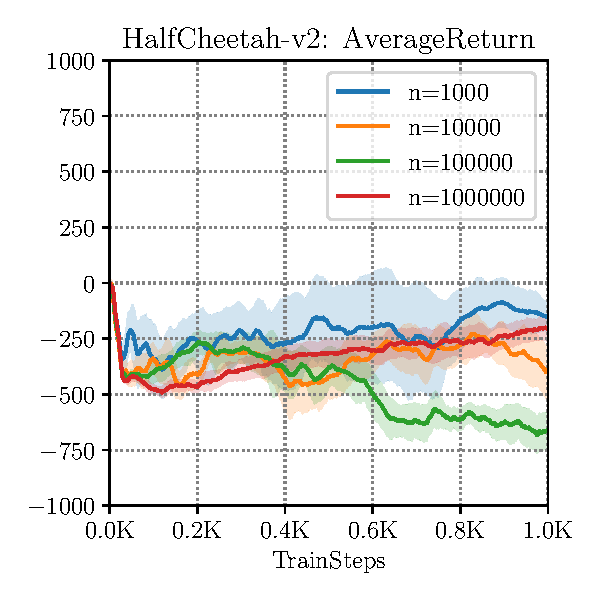
\includegraphics[width=0.45\linewidth]{chapters/bear/images/cheetah_divergence.pdf}
    ~
    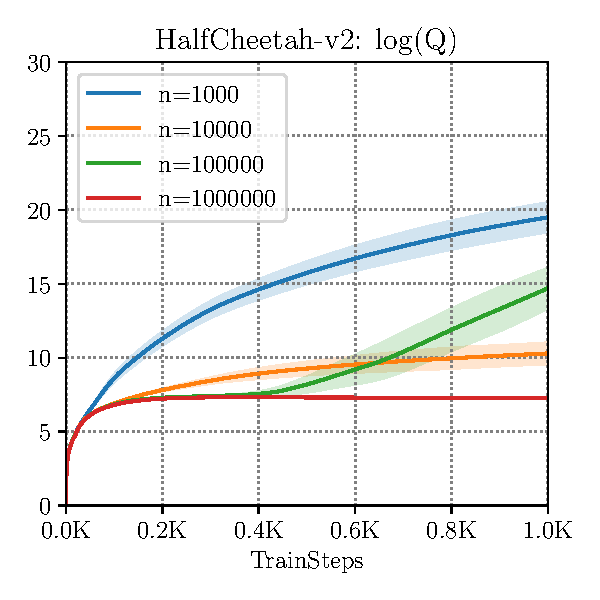
\includegraphics[width=0.45\linewidth]{chapters/bear/images/cheetah_divergence_q_val.pdf}
  \end{center}
 \vspace{-10pt}
 %%SL.5.22: Very important: the y-axes are not labeled right now, and it took me a while to figure out which plot was showing what. What is log(Q)? I guess you're trying to show that the right plot has Bellman error (?), while the left has performance? A couple more things: (1) always put space before ( (you often omit this space) (2) consider a caption like this (once the figures are labeled more clearly): Off-policy learning with SAC on HalfCheetah-v2 for different dataset sizes ($n$). The performance (left) does not correlate with $n$, while the Q-values (right) diverge or saturate at values far from the actual return.
  \caption{ \footnotesize Performance of SAC on HalfCheetah-v2 (return (left) and $\log$ Q-values (right)) with off-policy expert data w.r.t. number of training samples ($n$). Note the large discrepancy between returns (which are negative) and $\log$ Q-values (which have large positive values), which is not solved with additional samples.} 
 \vspace{-15pt}
 \label{fig:divergence}
\end{figure}
Building upon the discoveries presented in Chapter~\ref{chapter:diagnosing}, we have observed that Q-learning methods frequently struggle to learn from static, off-policy data, particularly in high-dimensional tasks. This difficulty is evident in Figure \ref{fig:divergence}. As outlined in the discussion of Chapter~\ref{chapter:diagnosing}, the primary cause of this instability lies in the challenges of handling distributional shift and statistical error. However, a crucial question remains: which factor plays a more significant role in this example? Furthermore, what mechanism underlies the emergence of this instability?

First of all, note that increasing the size of the static dataset does not rectify the problem (compare $n=1M$ vs $n=1000$), suggesting the issue in this setting is largely due to distributional shift. We can understand the source of this instability by examining the form of the Bellman backup. Although minimizing the mean squared Bellman error corresponds to a supervised regression problem, the targets for this regression are themselves derived from the current Q-function estimate. The targets are calculated by maximizing the learned $Q$-values with respect to the action at the next state. However, the $Q$-function estimator is only reliable on inputs from the same distribution as its training set. As a result, na\"{i}vely maximizing the value may evaluate the $\hat{Q}$ estimator on actions that lie far outside of the training distribution, resulting in pathological values that incur large error. We refer to these actions as out-of-distribution (OOD) actions. 

Formally, let $\valerr_k(\bs, \mathbf{a}) = |Q_k(\bs, \mathbf{a}) - Q^*(\bs, \mathbf{a})|$ denote the total error at iteration $k$ of Q-learning, and let $\projerr_k(\bs, \mathbf{a}) = |Q_k(\bs, \mathbf{a}) - \mathcal{B} Q_{k-1}(\bs, \mathbf{a})|$ denote the current Bellman error. Then, we have \mbox{$\valerr_k(\bs, \mathbf{a}) \le \projerr_k(\bs, \mathbf{a}) + \gamma \max_{\mathbf{a}'} \expec_{\bs'}[\valerr_{k-1}(\bs', \mathbf{a}')]$}. In other words, errors from $(\bs', \mathbf{a}')$ are discounted, then accumulated with new errors $\projerr_k(\bs, \mathbf{a})$ from the current iteration. We expect $\projerr_k(\bs, \mathbf{a})$ to be high on OOD states and actions, as errors at these state-actions are never directly minimized while training.

To mitigate bootstrapping error, we can restrict the policy to ensure that it output actions that lie in the support of the training distribution. This is distinct from previous work~\citep{jaques2019way} which implicitly constrains the \emph{distribution} of the learned policy to be close to the behavior policy, similarly to behavioral cloning~\cite{Schaal99isimitation}.
While this is sufficient to ensure that actions lie in the training set with high probability, it is overly restrictive. For example, if the behavior policy is close to uniform, the learned policy will behave randomly, resulting in poor performance, even when the data is sufficient to learn a strong policy (see Figure~\ref{fig:gridworld}
for an illustration). {Formally, this means that a learned policy $\pi(\mathbf{a}| \bs)$ has positive density\textit{ only where} the density of the behaviour policy $\beta(\mathbf{a}|s)$ is more than a threshold (i.e., $\forall \mathbf{a}, \beta(\mathbf{a}|\bs) \leq \varepsilon \implies \pi(\mathbf{a}|\bs) = 0$), instead of a closeness constraint on the value of the density $\pi(\mathbf{a}|\bs)$ and $\beta(\mathbf{a}|\bs)$.}
Our analysis instead reveals a tradeoff between staying within the data distribution and finding a suboptimal solution when the constraint is too restrictive. Our analysis motivates us to restrict the support of the learned policy, but not the probabilities of the actions lying within the support. This avoids evaluating the Q-function estimator on OOD actions, but remains flexible in order to find a performant policy. Our proposed algorithm leverages this insight. 

\vspace{-0.2cm}
\section{Formal Analysis and Distribution-Constrained Backups}
\label{sec:dist_constrained}
\vspace{-0.2cm}
In this section, we define and analyze a backup operator that restricts the set of policies used in the maximization of the Q-function, and we derive performance bounds which depend on the restricted set. This provides motivation for constraining policy support to the data distribution, allowing us to address the issue discussed above. We begin with the definition of a distribution-constrained operator:

\begin{tcolorbox}[colback=blue!6!white,colframe=black,boxsep=0pt,top=3pt,bottom=5pt]
\begin{definition}[Distribution-constrained operators]
Given a set of policies $\Pi$, the distribution-constrained backup operator is defined as:
%\[ \TPi Q(s, a) \coloneqq \expec \big[ R(s, a) + \gamma \expec_{\trans(s' | s, a)}\left[\max_{\pi \in \Pi} \expec_{\pi}[Q(s', a')] \right] \big] \]
\begin{align*}
\TPi Q(\mathbf{s}, \mathbf{a}) \defeq \expec \big[ R(\bs, \mathbf{a}) + \gamma \max_{\pi \in \Pi} \expec_{\trans(\bs' | \bs, \mathbf{a})}\left[V(\bs') \right] \big]
\ \ \ \ \ \ \ \ \ \ \ \ 
V(\bs) \defeq \max_{\pi \in \Pi} \expec_{\pi}[Q(\mathbf{s}, \mathbf{a})]\ \ .
\end{align*}
\end{definition}
\end{tcolorbox}
This backup operator satisfies properties of the standard Bellman backup, such as convergence to a fixed point, as discussed in Appendix~\ref{app:constrained_backup}. To analyze the (sub)optimality of performing this backup under approximation error, we first quantify two sources of error. The first is a \emph{suboptimality bias}. The optimal policy may lie outside the policy constraint set, and thus a suboptimal solution will be found. The second arises from distribution shift between the training distribution and the policies used for backups. This formalizes the notion of OOD actions. %and states.
To capture suboptimality in the final solution, we define a \emph{suboptimality constant}, which measures how far $\pi^*$ is from $\Pi$. 

\begin{definition}[Suboptimality constant]
The suboptimality constant is defined as:
\[ \alpha(\Pi) = \max_{\bs, \mathbf{a}} |\TPi Q^*(\bs, \mathbf{a}) - \backup Q^*(\bs, \mathbf{a})|. \]
\end{definition}
\vspace{-10pt}
Next, we define a concentrability coefficient~\citep{munos2005erroravi}, which quantifies how far the visitation distribution generated by policies from $\Pi$ is  from the training data distribution. This constant captures the degree to which states and actions are out of distribution.
\begin{tcolorbox}[colback=blue!6!white,colframe=black,boxsep=0pt,top=3pt,bottom=5pt]
\begin{assumption}[Concentrability]
Let $\rhoinit$ denote the initial state distribution, and $\mu(\bs, \mathbf{a})$ denote the distribution of the training data over $\mathcal{S} \times \mathcal{A}$, with marginal $\mu(\bs)$ over $\mathcal{S}$. Suppose there exist coefficients $c(k)$ such that for any $\pi_1, ... \pi_k \in \Pi$ and $s \in \mathcal{S}$:
\[
\rhoinit P^{\pi_1}P^{\pi_2}...P^{\pi_k}(s) \le c(k) \mu(\bs),
\]
where $P^{\pi_i}$ is the transition operator on states induced by $\pi_i$.
Then, define the concentrability coefficient $C(\Pi)$ as
\[
C(\Pi) \defeq (1-\gamma)^2\sum_{k=1}^\infty k\gamma^{k-1}c(k).
\] \label{assumption:conc} \end{assumption} 
\end{tcolorbox}
% \vspace{-10pt}
To provide some intuition for $C(\Pi)$, if $\mu$ was generated by a single policy $\pi$, and $\Pi = \{\pi\}$ was a singleton set, then we would have $C(\Pi)=1$, which is the smallest possible value. However, if $\Pi$ contained policies far from $\pi$, the value could be large, potentially infinite if the support of $\Pi$ is not contained in $\pi$. Now, we bound the performance of approximate distribution-constrained Q-iteration:

\begin{tcolorbox}[colback=blue!6!white,colframe=black,boxsep=0pt,top=3pt,bottom=5pt]
\begin{theorem}
\label{thm:avi_bound}
Suppose we run approximate distribution-constrained value iteration with a set constrained backup $\TPi$. Assume that $\delta(\bs,\mathbf{a}) \ge \max_k |Q_k(\bs, \mathbf{a}) - \TPi Q_{k-1}(\bs, \mathbf{a})|$ bounds the Bellman error. Then,
\[\lim_{k \to \infty} \expec_{\rhoinit}[|V^{\pi_k}(\bs) - V^*(\bs)|] \le
\frac{\gamma}{(1-\gamma)^2}\left[ C(\Pi)\expec_\mu[\max_{\pi \in \Pi} \expec_{\pi}[\projerr(\bs, \mathbf{a})]] + \frac{1-\gamma}{\gamma}\alpha(\Pi) \right]
\]
\end{theorem}
\end{tcolorbox}
\begin{proof} See Appendix~\ref{app:error_prop}, Theorem~\ref{thm:avi_bound_proof} \end{proof}
This bound formalizes the tradeoff between keeping policies chosen during backups close to the data (captured by $C(\Pi)$) and keeping the set $\Pi$ large enough to capture well-performing policies (captured by $\alpha(\Pi)$). When we expand the set of policies $\Pi$, we are increasing $C(\Pi)$ but decreasing $\alpha(\Pi)$. An example of this tradeoff, and how a careful choice of $\Pi$ can yield superior results, is given in a tabular gridworld example in Fig.~\ref{fig:gridworld}, where we visualize errors accumulated during distribution-constrained Q-iteration for different choices of $\Pi$. 

Finally, we motivate the use of support sets to construct $\Pi$. We are interested in the case where $\Pi_\epsilon = \{ \pi ~|~ \pi( \mathbf{a} | \bs) = 0 \text{ whenever } \beta( \mathbf{a} | \bs) < \epsilon \}$, where $\beta$ is the behavior policy (i.e., $\Pi$ is the set of policies that have support in the probable regions of the behavior policy). Defining $\Pi_\epsilon$ in this way allows us to bound the concentrability coefficient:

\begin{tcolorbox}[colback=blue!6!white,colframe=black,boxsep=0pt,top=3pt,bottom=5pt]
\begin{theorem}
\label{thm:conc_coeff_bound}
% Assume the data distribution $\mu$ is generated by a policy $\beta$, such that $\mu(s,a) = d_\beta(s,a)$. Let $\mu_\beta(s)$ be the state-visitation marginal for $\beta$. Let us define $\Pi_\epsilon = \{ \pi ~|~ \pi( a | s) = 0 \text{ whenever } \beta( a | s) < \epsilon \}$. Let $\mu_{\Pi}(s)$ be the maximum discounted visitation marginal of a state generated by some sequence of policies $\{\pi_i\}_{i} \in \Pi$ and let $f(\epsilon) \defeq \min_{s \in \mathcal{S}, \mu_\Pi(s) > 0} [\mu(s)]$. Then, Assumption~\ref{assumption:conc} is satisfied for a $C(\Pieps)$ that is bounded as:
% \[
% C(\Pi_\epsilon) \leq C(\beta) \cdot \Big(1 + \frac{\gamma}{(1 - \gamma) f(\epsilon)} (1 - \epsilon)\Big)
% \]
Assume the data distribution $\mu$ is generated by a behavior policy $\beta$. %, such that $\mu(s,a) = d_\beta(s,a)$. 
Let $\mu(\bs)$ be the marginal state distribution under the data distribution. Define $\Pieps = \{ \pi ~|~ \pi( \mathbf{a} | \bs) = 0 \text{ whenever } \beta( \mathbf{a} | \bs) < \epsilon \}$ and let $\mu_\Pieps$ be the highest discounted marginal state distribution starting from the initial state distribution $\rho$ and following policies $\pi \in \Pieps$ at each time step thereafter. Then, there exists a concentrability coefficient $C(\Pieps)$ which is bounded:
\[
C(\Pi_\epsilon) \leq C(\beta) \cdot \Big(1 + \frac{\gamma}{(1 - \gamma) f(\epsilon)} (1 - \epsilon)\Big)
\]
where $f(\epsilon) \defeq \min_{\bs \in \mathcal{S}, \mu_\Pieps(\bs) > 0} [\mu(\bs)] > 0$.
\end{theorem}
\end{tcolorbox}
% \vspace{-10pt}
\begin{proof} See Appendix~\ref{app:error_prop}, Theorem~\ref{thm:conc_coeff_proof} \end{proof}
% \vspace{-10pt}
Qualitatively, $f(\epsilon)$ is the minimum discounted visitation marginal of a state under the behaviour policy if only actions which are more than $\epsilon$ likely are executed in the environment. Thus, using support sets gives us a single lever, $\epsilon$, which simultaneously trades off the value of $C(\Pi)$ and $\alpha(\Pi)$. Not only can we provide theoretical guarantees, we will see in our experiments (Sec.~\ref{sec:experiments}) that constructing $\Pi$ in this way provides a simple and effective method for implementing distribution-constrained algorithms. 

Intuitively, this means we can prevent an increase in overall error in the Q-estimate by selecting policies supported on the support of the training action distribution, which would ensure roughly bounded projection error $\delta_k(\mathbf{s}, \mathbf{a})$ while reducing the suboptimality bias, potentially by a large amount. Bounded error $\delta_k(\bs, \mathbf{a})$ on the support set of the training distribution is a reasonable assumption when using highly expressive function approximators, such as deep networks, especially if we are willing to reweight the transition set~\cite{Schaul2015,fu2019diagnosing}. We further elaborate on this point in Appendix~\ref{app:bearql-more}.

\begin{figure}
    \centering
    \vspace{-0.1in}
    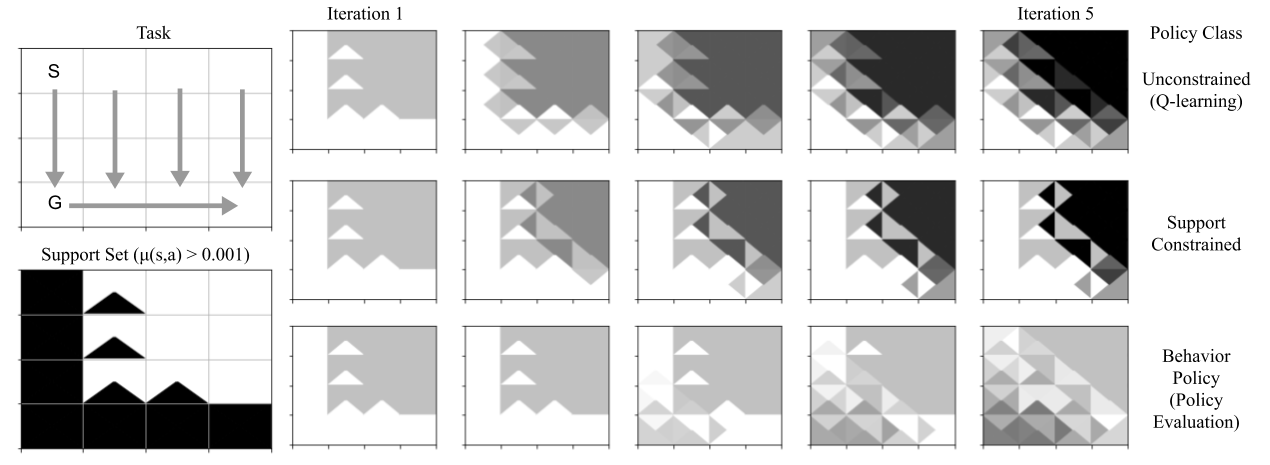
\includegraphics[width=0.9\textwidth]{chapters/bear/images/gridworld}
    \caption{ \footnotesize Visualized error propagation in Q-learning for various choices of the constraint set $\Pi$:
    unconstrained (top row) distribution-constrained (middle),
    and constrained to the behavior policy (policy-evaluation, bottom). Triangles represent Q-values for actions that move in different directions. The task (left) is to reach the bottom-left corner (G) from the top-left (S), but the behaviour policy (visualized as arrows in the task image, support state-action pairs are shown in black on the support set image) travels to the bottom-right with a small amount of $\epsilon$-greedy exploration. Dark values indicate high error, and light values indicate low error. Standard backups propagate large errors from the low-support regions into the high-support regions, leading to high error. Policy evaluation reduces error propagation from low-support regions, but introduces significant suboptimality bias, as the data policy is not optimal. A carefully chosen distribution-constrained backup strikes a balance between these two extremes, by confining error propagation in the low-support region while introducing minimal suboptimality bias.}
    \label{fig:gridworld}
    \vspace{-0.1in}
\end{figure}

% \subsection{Choosing Backup Policies for OOD Action Error Reduction}
% \label{sec:choosing_policies}
% Argument in Sec.~\ref{sec:tradeoff} tells us that, with a careful selection of the policy under which the target value is computed, the overall error of value estimates from the optimal value function $\|V^* - V_k\|$ can be reduced. How should we search for a policy that minimizes the overall error? Our choice is to backup from policies which maintain high-support over the action set of the data.
% %%SL.5.22: I think it's not obvious to readers that "policy for the backup" means the distribution over the actions under which the target value is calculated. -- addressed

% To justify this choice,
% %%SL.5.22: What choice? -- choice of backing up from any policy that maintains high support over data.
% we note that the error analysis relies on being able to quantify $\delta_k(s, a)$ (the per-state-action bellman error) for OOD actions. Outside of the support of the data distribution, it is hard to provide guarantees on $\delta_k$. However, when $a$ lies inside the support of the training distribution for a given state $s$, high-capacity function approximators trained with supervised learning are expected to produce a bounded error, given enough samples.
% %Even if they don't produce bounded error on such in-support inputs, techniques such as Prioritized Replay~\cite{Schaul2016PrioritizedER} can be employed to ensure bounded error on all in-support inputs. 
% %Furthermore, often the quantity of interest is the Bellman error weighted by the inverse density of the behaviour policy~\cite{antos07fitted}, which depends only on the support of the behaviour policy and this error metric is the equal for two policies provided they share the same support.
% Therefore, backing up from all actions that have non-negligible support under the training distribution is sufficient (but not necessary) to prevent error accumulation. Hence, we restrict the set $\Pi$
% %%SL.5.22: Did we define \Pi before? since we cut the set backup operator stuff, now this is much harder to follow. Maybe we can bring it back (but call it something else)?
% of policies used for distribution-constrained backups to the set of policies that are supported on the probable regions of the behaviour policy. That is, $\Pi = \{ \pi | \pi( a | s) = 0 \text{ whenever } \beta( a | s) < \epsilon \}$, where $\beta$ is the behavior policy (i.e., the set of policies that have support in the probable regions of the behavior policy). This means that we are allowed to backup from any action distribution supported over the support of the behaviour policy. Previous work~\cite{fujimoto2018off} restricts the choice of actions to be a distribution close to the behaviour policy. 

%%SL.5.22: I don't really understand what the above paragraph is saying. Read literally, it seems to say "prior work does something similar, and in the worst case we are equally bad." That's not very satisfying. Maybe just delete this paragraph, or rephrase if that's not what you meant?
%Now, explain why this does a good job of balancing the terms. Next, we explain how this bound motivates the use of set-constrained backups to reduce accumulation of bootstrapping error. \TODO{explanation about $\delta1$ goes here} -- addressed -- removed this paragraph


% we need to determine how to formulate the appropriate constraint and how to implement so as to back up only values of policies in $\Pi$.
% %%SL.5.20: Rephrase. In order to develop a practical algorithm based on the set-constrained backup, we need to determine how to formulate the appropriate constraint and how to implement so as to back up only values of policies in $\Pi$.
% Intuitively, we would like $\Pi(s)$ for a particular state $s$ to contain only those policies that permit actions within the support of the dataset distribution. Instead of inferring $\Pi$, we use a notion of divergence between the uniform distribution over the support-set of the current policy and the current policy for optimization.  

% %%SL.5.20: Rephrase. Intuitively, we would like $\Pi(s)$ for a particular state $s$ to contain only those policies that permit actions withi
% In order confidence support set perform the $\max$ on the high-over actions from only these policies, we need to define a tractable objective. Instead of inferring the set of policies $\Pi$ we rather resort to specifying a notion of divergence between the set $\mathcal{A}_\varepsilon^\dataset$ and the current policy, $\operatorname{Divergence}(\mathcal{A}^{\mathcal{D}}_{\varepsilon}(s), \pi)$ thereby fitting the problem of inferring $\Pi$ in an optimization setup.
% %%SL.5.20: I don't really understand the above sentence. Try rewriting it to be clearer?
% Next, we move on to presenting our method, which we call \emph{bootstrap error accumulation reduction} (BEAR).

\vspace{-0.2cm}
\section{Bootstrapping Error Accumulation Reduction (BEAR)}
\label{sec:bear}
\vspace{-0.2cm}

% \vspace{-0.1in}
We now propose a practical actor-critic algorithm (built on the framework of TD3~\cite{fujimoto18addressing} or SAC~\cite{haarnoja2018sac}) that uses distribution-constrained backups to reduce accumulation of bootstrapping error. The key insight is that we can search for a policy with the same support as the training distribution, while preventing accidental error accumulation.
Our algorithm has two main components. Analogous to BCQ~\citep{fujimoto18addressing}, we use $K$ Q-functions and use the minimum Q-value for policy improvement, and design a constraint which will be used for searching over the set of policies $\Pieps$, which share the same support as the behavior policy. Both of these components will appear as modifications of the policy improvement step in actor-critic style algorithms. We also note that policy improvement can be performed with the mean of the K Q-functions, and we found that this scheme works as good in our experiments. 

% n components. Analogous to BBCQ~\citep{fujimoto2018off}, we use two Q-functions and linearly combine their predictions the Q-function for policy improvement, and design a constraint which will be used for searching over the set of policies $\Pieps$, which share the same support as the behaviour policy. Both of these components will appear as modifications of the policy improvement step in actor-critic style algorithms.

We denote the set of Q-functions as: $\hat{Q}_1, \cdots, \hat{Q}_K$.
% compute a conservative estimate of the Q-values: $\frac{1}{K} \sum_{i=1}^K \hat{Q}_i (s, a) - \lambda \sqrt{\operatorname{var}_k \hat{Q}_k(s, a)}$, where $\lambda \in \mathbb{R}^+$ is a hyperparameter. %We use this value as a conservative estimate of the Q-function. This can be derived using Cantelli's inequality. 
Then, the policy is updated to maximize the conservative estimate of the Q-values within $\Pieps$: 
% \vspace{-10pt}
$$ \pi_\phi(\bs) := \max_{\pi \in \Pieps} \expec_{a \sim \pi(\cdot|\bs)} \left[\min_{j=1,..,K} \hat{Q}_j(\bs, \mathbf{a})\right] $$
% \lambda \sqrt{ \operatorname{var_k}\expec_{a \sim \pi(\cdot |s) }[\hat{Q}_k(s, a)]}.$$
% \vspace{-5pt}
% Let $\mathcal{F}_t$ be the sigma-algebra generated by the training procedure until iteration $t$, and let $\operatorname{var}_{t} \hat{Q}(s,a) := \mathbb{E}[(\hat{Q}_t(s, a) - \mathbb{E}[(\hat{Q}_t(s, a) | \mathcal{F}_t))^2|\mathcal{F}_t]$
%%SL.5.20: use mbox. And for clarity, it might be good to indicate what the expectation is over (and use [ instead of ( for E so that parens don't get cluttered). Also, what is up with this (s,a) hanging out at the end? do you mean to put (s,a) inside (after \hat{Q})?
% denote the variance of the Q-function $\hat{Q}_t$, at time $t$ during training. Then, for each state-action pair $(s, a)$, 
% ${Pr (\hat{Q}_t \geq \mathbb{E}(\hat{Q}_t|\mathcal{F}_t) + \sqrt{\frac{(1 - \delta) \operatorname{var}_{t} \hat{Q}_t }{\delta}})  \leq \delta}$
%%SL.5.20: can you state in words what this means for the purpose of this section? also, rhetoric-wise, amybe better state as a theorem (it's kind of obvious, but still) and then after say that this is easy to show via Cantelli's inequality or something?

%%SL.5.20: It's not clear what the concentration bound is actually used for.

 %In the above concentration bound, $\mathbb{E}(\hat{Q}_t|\mathcal{F}_t)$ refers to the true Q-value, which can be obtained given no stochasticity in the procedure.


%%SL.5.20: The logical thread here is broken. What are you doing with set divergence? State the issue first, then th e resolution, else it's hard for the reader to follow.
In practice, the behavior policy $\beta$ is unknown, so we need an approximate way to constrain $\pi$ to $\Pi$. We define a differentiable constraint that approximately constrains $\pi$ to $\Pi$, and then approximately solve the constrained optimization problem via dual gradient descent.  We use the sampled version of maximum mean discrepancy (MMD)~\cite{gretton2012kernel}
%%SL.5.22: Alg names are not capitalized unless they contain proper nouns, put a space after the words and before open paren (I fixed it above, but this issue happens often, please take this comment into account) -- Thanks for pointing this out!
between the unknown behavior policy $\beta$ and the actor $\pi$ because it can be estimated based solely on samples from the distributions. Given samples $x_1, \cdots, x_n \sim P$ and $y_1, \cdots, y_m \sim Q$, the sampled MMD between $P$ and $Q$ is given by:\\
$$\operatorname{MMD}^2(\{x_1, \cdots, x_n\}, \{y_1, \cdots, y_m\}) = \frac{1}{n^2} \sum_{i, i'} k(x_i, x_{i'}) - \frac{2}{nm} \sum_{i, j} k(x_i, y_j) + \frac{1}{m^2} \sum_{j, j'} k(y_j, y_{j'}).
$$
Here, $k(\cdot, \cdot)$ is any universal kernel. In our experiments, we find both Laplacian and Gaussian kernels work well.
%As the $\operatorname{MMD}$ distance does not depend on the density function of either distribution, minimizing it using samples is a reasonable proxy for enforcing that $Q$ lies inside the support of $P$. This is because, 
The expression for MMD does not involve the density of either distribution and it can be optimized directly through samples. Empirically we find that, in the low-intermediate sample regime, the sampled MMD between $P$ and $Q$ is similar to the MMD between a uniform distribution over $P$'s support and $Q$, which makes MMD roughly suited for constraining distributions to a given support set. (See Appendix~\ref{app:mmd} for numerical simulations justifying this approach).

% and hence, we parameterize the set $\mathcal{A}^{\mathcal{D}}_{\varepsilon}(s)$ as a distribution $\pi_{set}(a|s)$ such that $\mathcal{A}(s) := \mathcal{A}^{\pi_{set}}_{\varepsilon}(s) := \{a \in \mathcal{A} | \pi_{set}(a|s) \geq \varepsilon \}$, in other words, $\mathcal{A}(s)$ is the high-confidence support set of the distribution $\pi_{set}$, and we train for a parametric $\pi_{set}$.
%%SL.5.20: I don't actually understand at this point what you are doing. Are you optimizing a neural net that denotes \pi_set? or something else?

% \paragraph{Deriving the update:} Let $\hat{Q}_k$ be the Q-function at the k-th step of the algorithm. Actor-critic Q-learning algorithms maintain a parameterized policy, $\pi_k$ that is updated towards the maximizing the Q-function.
% %-- $\pi_{k+1}(s) := \max_{\pi \in \Delta_{|S|}} E_{a \sim \pi(\cdot|s)} [\hat{Q}_{k}(s, a)]$. 
% In order to reduce the number of moving parts, we let the actor in this case serve both its regular function of maximizing the Q-function while also constraining the action distribution close to $\mathcal{A}^\dataset_\varepsilon$, which is the the task of $\pi_{set}$. We use the bound derived on Q-values to update the policy in the direction of maximizing a conservative estimate of the true Q-value -- $$ \pi_{k+1}(s) := \max_{\pi \in \Delta_{|S|}} E_{a \sim \pi(\cdot|s)} [\hat{Q}_{k}(s, a)] - \lambda \sqrt{ \operatorname{var_k}E_{a \sim \pi(\cdot |s) }[\hat{Q}_k(s, a)]}$$
% %TODO{may want to mention that this amounts to subtracting a constant times the std, which sounds reasonable}
% We still need to account for the problem of specifying support divergence. In order to enforce this constraint, we use a measure of support matching between the training distribution $\Pi$ and the policy $\pi(\cdot|s)$, which we choose to be a sampled version of the Maximum Mean Discrepancy(MMD) Distance between $\Pi$ and the actor $\pi$. Sampled MMD distance between two probability distributions $P$ and $Q$ is given by, $\operatorname{MMD}(P, Q)$, where $x_1, \cdots, x_n \sim P$ and $y_1, \cdots, y_m \sim Q$ is given by:\\
% $$\operatorname{MMD}^2(\{x_1, \cdots, x_n\}, \{y_1, \cdots, y_m\}) = \frac{1}{n^2} \sum_{i, i'} k(x_i, x_{i'}) - \frac{2}{nm} \sum_{i, j} k(x_i, y_j) + \frac{1}{m^2} \sum_{j, j'} k(y_j, y_{j'})
% $$
% When the number of samples $n$ is an intermediate number (4-10), the above sampled objective can also be approximately considered as a distance between a uniform distribution over the high confidence support set of the distribution $P$ and the distribution $Q$ -- therefore, if trained perfectly, $Q$ should have the same support as $P$. That is, $\operatorname{MMD}(P, Q)$ is a reasonable proxy for $\operatorname{MMD}(\mathcal{U}(\mathcal{A}_{\varepsilon}(P)), Q)$. 
% %\TODO{what does it mean MMD between a set and distribution}
% The expression for $\operatorname{MMD}$ does not use the density function of either distribution, thereby making it suited as an approximate way of support matching.

Putting together, the optimization problem in the policy improvement step is
% \vspace{-5pt}
\begin{multline}
    \label{eqn:policy_update}
   \pi_\phi := \max_{\pi \in \Delta_{|S|}} \expec_{\bs \sim \mathcal{D}} \expec_{\mathbf{a} \sim \pi(\cdot|\bs)} \left[\min_{j=1,..,K} \hat{Q}_j(\bs, \mathbf{a})\right] 
%   - \lambda \sqrt{ \operatorname{var_k}\expec_{a \sim \pi(\cdot |s) }[\hat{Q}_k(s, a)]}\\
   \text{~~s.t.~~} \mathbb{E}_{\bs \sim \mathcal{D}} [\operatorname{MMD}(\mathcal{D}(\bs), \pi(\cdot|\bs))] \leq \varepsilon \quad
\end{multline}
where $\varepsilon$ is an approximately chosen threshold. We choose a threshold of $\varepsilon=0.05$ in our experiments. The algorithm is summarized in Algorithm~\ref{algo:bear_ql}. 
% Step 5 of the algorithm performs a stochastic version of the distribution-constrained backup, where Dirac-delta policies $\delta_{a_i}, \cdots, \delta_{a_p},(~\forall~i, \delta_{a_i} \in \Pi)$ are sampled, an expectation of the target Q-value under these Dirac-delta policies is computed and then the maximum value across these policies is backed up as defined by the backup operator. We provide more explanation in Appendix \ref{app:bearql-more}.

\textbf{How does BEAR connect with distribution-constrained backups described in Section 4.1?} Step 5 of the algorithm restricts $\pi_\phi$ to lie in the support of $\beta$. This insight is formally justified in Theorems 4.1 \& 4.2 ($C(\Pi_\varepsilon)$ is bounded). Computing distribution-constrained backup exactly by maximizing over $\pi \in \Pi_\varepsilon$ is intractable in practice. As an approximation, we sample Dirac policies in the support of $\beta$ (Alg 1, Line 5) and perform empirical maximization to compute the backup. As the maximization is performed over a \textit{narrower} set of Dirac policies ($\{ \delta_{\mathbf{a}_i} \} \subseteq \Pi_\varepsilon$), the bound in the above Theorem still holds. Empirically, we show in Section~\ref{sec:experiments} that this approximation is sufficient to outperform previous methods. This connection is briefly discussed in Appendix~\ref{app:bear_dist_constrained}.
% $\operatorname{var}(\hat{Q}_k(s, a)) \approx \frac{1}{M} \sum_{i=1}^{M} (\hat{Q}_{\theta_i, k}(s, a) - \bar{Q}_{\theta, k}(s, a))^2$, where $\bar{Q}_{\theta, k}(s, a) = \frac{1}{M} \sum_{i=1}^{M} \hat{Q}_{\theta_i, k}(s, a)$ is the sample mean of the ensemble. 

%AK.05.15: Note to Sergey: this is the actor-critic version, optional depends on results.
% Another variant of the above approach can be where this single policy improvement step can be decomposed into two decoupled steps -- (1) Learning a policy $\pi_{set}$, whose high-confidence set defines the support set $\mathcal{A}_{\varepsilon}(s)$ at a state $s$, by minimizing the sampling error in $\hat{Q}_k$ and accounting for the deviation from the dataset, and then, (2) Learning to maximize the expected Q-function $\hat{Q}_k$ on this set $\mathcal{A}_{\varepsilon}(s)$, in practice obtained by sampling from $\pi_{set}$. In practice, we found using Equation~\ref{eqn:policy_update} working better than the latter approach and hence, we stick to this formulation for our experiments. The overall algorithm is summarized in Algorithm~\ref{alg:q_learning}, and the actor-critic version is described in Algorithm~\ref{alg:actor_critic}.   
% \vspace{-5pt}
\begin{algorithm}[h]
\small
\caption{Q-learning variant of BEAR (BEAR)}
\label{alg:q_learning}
\begin{algorithmic}[1]
    \State Dataset $\mathcal{D}$, target network rate $\tau$, batch size $N$, sampled actions for MMD $n$, minimum $\lambda$
    \State Initialize Q-ensemble $\{Q_{\theta_i} \}_{i=1}^{K}$, actor $\pi_{\phi}$, multiplier $\alpha$, target networks $\{ Q_{\theta'_i} \}_{i=1}^K$, and a target actor $\pi_{\phi'}$, with $\phi' \leftarrow \phi, \theta'_i \leftarrow \theta_i$
    \ForAll{$t$ in \{1, \dots, N\}}
        \State Sample mini-batch of transitions $(\bs, \mathbf{a}, r, \bs') \sim \mathcal{D}$\\
        \textbf{Q-update:}
            \State Sample $p$ action samples, $\{\mathbf{a}_i \sim \pi_{\phi'}(\cdot|\bs')\}_{i=1}^p$
            \State Define $y(\bs, \mathbf{a}) := \max_{\mathbf{a}_i} [ \lambda \min_{j=1,..,K} Q_{\theta'_j}(\bs', \mathbf{a}_i) + (1 - \lambda) \max_{j=1,..,K} Q_{\theta'_j}(\bs', \mathbf{a}_i)]$
            \State $\forall i, \theta_i \leftarrow \arg \min_{\theta_i} (Q_{\theta_i}(\bs, \mathbf{a}) - (r + \gamma y(\bs, \mathbf{a})))^2$\\
        \textbf{Policy-update:}
        \State Sample actions $\{ \hat{\mathbf{a}}_i \sim \pi_{\phi}(\cdot | \bs) \}_{i=1}^{m}$ and $\{ \mathbf{a}_j \sim \mathcal{D}(\bs)\}_{j=1}^{n}$. % $n$ preferably an intermediate integer(1-10)
        \State Update $\phi$, $\alpha$ by minimizing Equation~\ref{eqn:policy_update} with Lagrange multiplier $\alpha$.
        \State \textbf{Update Target Networks: } $\theta'_i \leftarrow \tau \theta_i + (1 - \tau)\theta'_i$; $\phi' \leftarrow \tau \phi + (1 -\tau) \phi'$ 
    \EndFor
\end{algorithmic}
\label{algo:bear_ql}
\end{algorithm}

In summary, the actor is updated towards maximizing the Q-function while still being constrained to remain in the valid search space defined by $\Pieps$. The Q-function uses actions sampled from the actor to then perform distribution-constrained Q-learning, over a reduced set of policies. {At test time, we sample $p$ actions from $\pi_\phi(\bs)$ and the Q-value maximizing action out of these is executed in the environment.}  %The maximization step in the actor-update empirically helps, but can be coupled with maximization in Step 5. Similar to \cite{fujimoto2018off} we use a soft-minimum to compute target values for updating Q-functions. 
Implementation and other details are present in Appendix \ref{app:bear_additional_details}.
%%SL.5.22: Remember to fill this in.

% \begin{algorithm}[H]
% \small
% \caption{BEAR Actor-Critic}
% \label{alg:actor_critic}
% \begin{algorithmic}[1]
%     \INPUT: Dataset $\mathcal{D}$, target network update rate $\tau$, mini-batch size $N$, sampled actions for MMD $n$, minimum $\lambda$, policy gradient clipping constants $\beta_1, \beta_2; \beta_1 \leq \beta_2$, MMD threshold constant $\varepsilon$
%     \STATE Initialize Q-ensemble $\{Q_{\theta_i} \}_{i=1}^{M}$, actor $\pi_{\phi}$, set-determining policy $\pi_{set}$, Lagrange multiplier $\alpha$, target networks $\{ Q_{\theta'_i} \}_{i=1}^M$, and a target actor $\pi_{\phi'}$, with $\phi' \leftarrow \phi, \theta'_i \leftarrow \theta_i$
%     \FOR{$t$ in \{1, \dots, N\}}
%         \STATE Sample mini-batch of transitions $(s, a, r, s') \sim \mathcal{D}$\\
%         \textbf{Q-update:}
%             \STATE Sample $m$ action samples, $\{a_i \sim \pi_{\phi'}(\cdot|s')\}_{i=1}^n$
%             \STATE Define $y = \frac{1}{m} \sum_{a_i} [ \lambda \min_{j=1,..,M} Q_{\theta'_j}(s', a_i) + (1 - \lambda) \max_{j=1,..,M} Q_{\theta'_j}(s', a_i)]$
%             \STATE $\forall i, \theta_i \leftarrow \arg \min_{\theta_i} (Q_{\theta_i}(s, a) - (r + \gamma y))^2$\\
%         \textbf{Set-update and Actor-update:}
%         \STATE Sample actions $A_1(s) \equiv \{ \hat{a}_i \sim \pi_{set}(\cdot | s) \}_{i=1}^{m}$ and $A_2(s) \equiv \{ a_j \sim \mathcal{D}(s)\}_{j=1}^{n}$, $n << m$
%         \STATE Update $\pi_{set}, \alpha$: $$ \pi_{set}, \alpha \leftarrow \arg \min_{\pi_{set}} \max_{\alpha \geq 0} \sqrt{\frac{(1 - \delta) \operatorname{var_k}E_{a \sim \pi_{set}(\cdot |s) }[\hat{Q}_k(s, a)]}{\delta}} + \alpha \mathbb{E}_{s \sim \mathcal{D}} ([\operatorname{MMD}(A_1, A_2)] -  \varepsilon) $$
%         \STATE Update $\phi$ using Importance Sampled Policy Gradient: 
%         $$ \pi_{\phi} \leftarrow  \max_{\pi_{\phi}} \mathbb{E}_{s \sim \mathcal{D}} \mathbb{E}_{a \sim \pi_{set}(\cdot|s)} \Big( \Big[ \frac{\pi_\phi(a|s)}{\pi_{set}(a|s)} \Big]_{\beta_1}^{\beta_2} Q(s, a) \Big)$$
%         \STATE \textbf{Update Target Networks: } $\theta'_i \leftarrow \tau \theta_i + (1 - \tau)\theta'_i$; $\phi' \leftarrow \tau \phi + (1 -\tau) \phi'$ 
%     \ENDFOR
% \end{algorithmic}
% \end{algorithm}


% Let $\bar{Q}(\cdot, \cdot)$ be the delayed target network, and $Q(\cdot, \cdot)$ be the current Q-function. Define $d_i$ be the the TD error for the $i^{th}$ datapoint.
% $$
% d_{i}(Q ; \bar{Q}, \pi)=R_{t}+\gamma \bar{Q}\left(s'_{i}, \pi_{set} \left(s'_i\right)\right)-Q\left(s_{i}, a_{i}\right)

% $$
% Further we define the empirical loss function by
% $$
% \hat{L}_{N}(Q ; \bar{Q}, \pi)=\frac{1}{N} \sum_{t=1}^{N} \frac{d_{t}^{2}(Q ; \bar{Q}, \pi_{set})}{\lambda(\mathcal{A})}
% $$
% where normalization $\lambda{\mathcal{A}}$ is introduced for mathematical convenience. Then, each policy evaluation step can be written as:  

% If we solely backup from actions present in our dataset, there is no way the algorithm can perform better than the policy that collected the data. The capacity of Q-learning and other ADP algorithms to ``stitch'' together performant sub-trajectories is lost. Hence, our method does allow the agent to backup from actions that occur outside the dataset, while still being constrained to not go farther away from the support of $\mathcal{D}$. In principle, a measure of distance from a given dataset can only be obtained using Bayesian Approaches (?). In practice, we use the variance of the ensemble as a measure to approximately quantify closeness to the support set. Our overall approach is described in the next paragraph.




% Our problem setting does not allow any interaction with the environment, and only lets us use the dataset $\mathcal{D}$. Since we see a limited subset of state-action pairs from the environment, the expected estimate of the Q-function conditioned on all training history in our case, $\mathbb{E}(\hat{Q}|\mathcal{F}_t)$, is biased. \TODO{aviral: finish this argument} 

% We train an ensemble of $N$ parametric Q-functions, $Q_{\theta_1}, \cdots, Q_{\theta_N}$ by using bootstrap masks on the data points of the dataset $\mathcal{D}$. This is done to simulate epistemic variance. To make sure that the actions chosen for backing up Q-functions are valid, we learn a set selection policy, $\pi_{set}$ -- a policy that can provide high densities to actions that don't propagate errors.   
% \section{Experimental Evaluation}
\label{sec:experiments}
In our experiments, we study how BEAR performs when learning from static offline data on a variety of continuous control benchmark tasks. We evaluate our algorithm in three settings: when the dataset $\dataset$ is generated by \textbf{(1)} a completely random behavior policy, \textbf{(2)} a partially trained, medium scoring policy, and \textbf{(3)} an optimal policy. Condition \textbf{(2)} is of particular interest, as it captures many common use-cases in practice, such as learning from imperfect demonstration data (e.g., of the sort that are commonly available for autonomous driving~\cite{DBLP:conf/iclr/GaoXLYLD18}), or reusing previously collected experience during off-policy RL. We compare our method to several prior methods: a baseline actor-critic algorithm (TD3), the BCQ  algorithm~\citep{fujimoto2018off}, which aims to address a similar problem, as discussed in Section~\ref{sec:Problem Description}, KL-control~\citep{jacques19way} (which solves a KL-penalized RL problem similarly to maximum entropy RL), a static version of DQfD~\citep{hester2018dqfd} (where a constraint to upweight Q-values of state-action pairs observed in the dataset is added as an auxiliary loss on top a regular actor-critic algorithm), and a behavior cloning (BC) baseline, which simply imitates the data distribution. This serves to measure whether each method actually performs effective RL, or simply copies the data. We report the average evaluation return over 5 seeds of the policy given by the learned algorithm, in the form of a learning curve as a function of number of gradient steps taken by the algorithm. These samples are only collected for evaluation, and are not used for training.

\subsection{Performance on Medium-Quality Data}

We first discuss the evaluation of condition with ``mediocre'' data \textbf{(2)}, as this condition resembles the settings where we expect training on offline data to be most useful. We collected one million transitions from a partially trained policy, so as to simulate imperfect demonstration data or data from a mediocre prior policy.
In this scenario, we found that BEAR consistently outperforms BCQ~\cite{fujimoto2018off} and a na\"ive off-policy RL baseline (TD3) (by large margins), as shown in Figure~\ref{fig:mediocre}. This scenario is the most relevant from an application point of view, as access to optimal data may not be feasible, and random data might have inadequate exploration to efficient learn a good policy. We also evaluate the accuracy with which the learned Q-functions predict actual policy returns. These trends are provided in Appendix~\ref{app:q_vs_mc}. 
% Note that the performance of BCQ often tracks the performance of the BC baseline, suggesting that BCQ primarily imitates the data. 
Our KL-control baseline uses automatic temperature tuning~\citep{haarnoja2018sac}. We find that KL-control usually performs similar or worse to BC, whereas DQfD tends to diverge, and often exhibits a huge variance across different runs (for example, HalfCheetah-v2 environment).  

\begin{figure}
    \centering
    \begin{subfigure}[t]{0.23\textwidth}
        \centering
        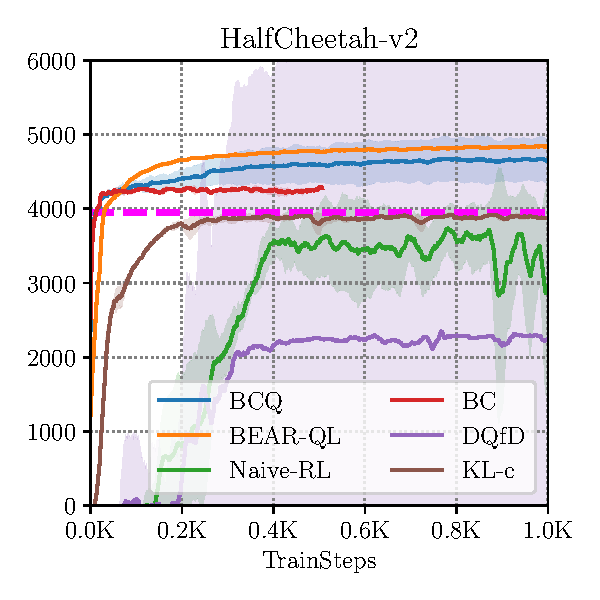
\includegraphics[width=0.99\linewidth]{chapters/bear/images/images_camera_ready/cheetah_mediocre_camera_ready.pdf}
    \end{subfigure}
    \begin{subfigure}[t]{0.23\textwidth}
        \centering
        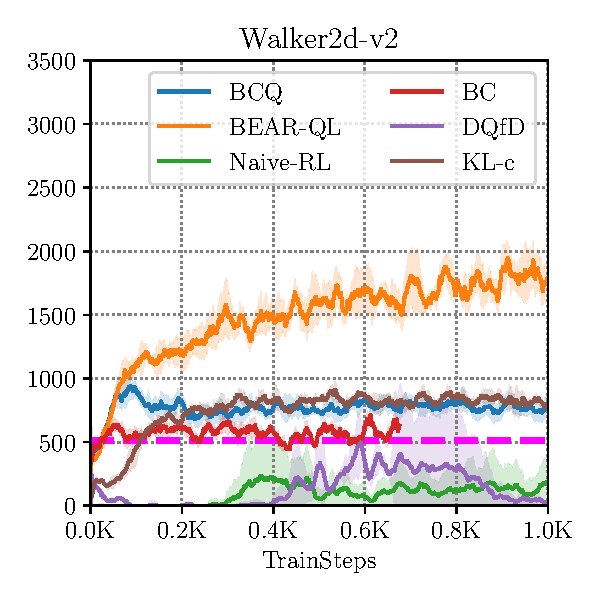
\includegraphics[width=0.99\linewidth]{chapters/bear/images/images_camera_ready/walker_mediocre_camera_ready.pdf}
        % \caption{}
    \end{subfigure}
    ~
    \begin{subfigure}[t]{0.23\textwidth}
        \centering
        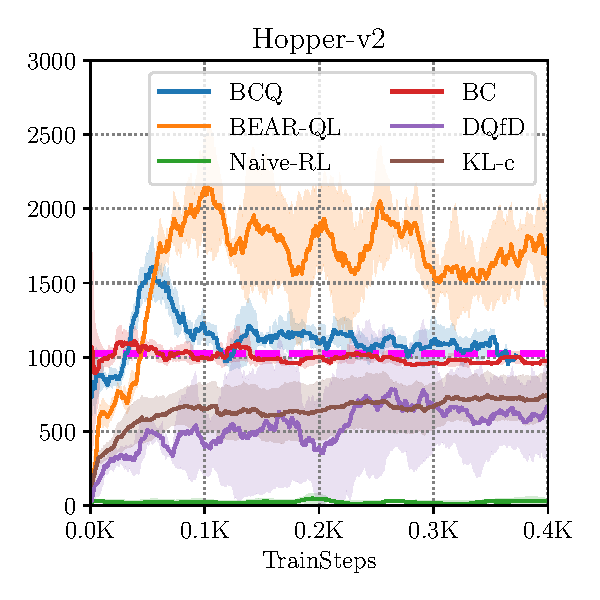
\includegraphics[width=0.99\linewidth]{chapters/bear/images/images_camera_ready/hopper_mediocre_camera_ready.pdf}
        % \caption{}
    \end{subfigure}
    ~
    \begin{subfigure}[t]{0.23\textwidth}
        \centering
        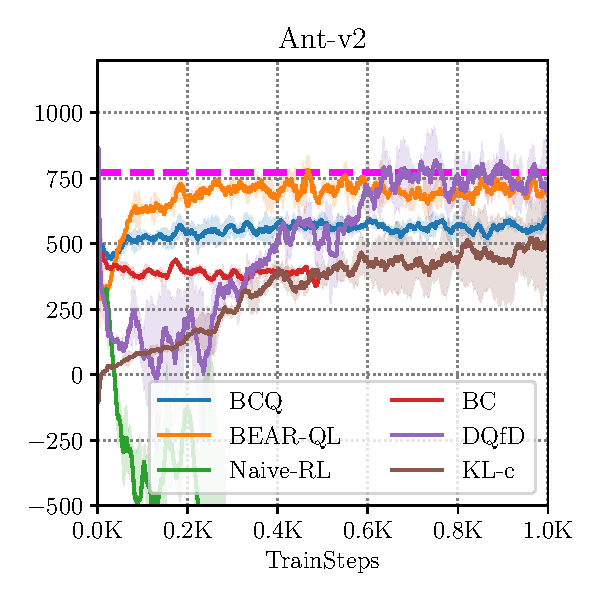
\includegraphics[width=0.99\linewidth]{chapters/bear/images/images_camera_ready/ant_mediocre_camera_ready.pdf}
        % \caption{}
    \end{subfigure}
    \caption{\label{fig:mediocre} \footnotesize Average performance of BEAR, BCQ, Na\"ive RL and BC on medium-quality data averaged over 5 seeds. BEAR outperforms both BCQ and Na\"ive RL. Average return over the training data is indicated by the magenta line. One step on the x-axis corresponds to 1000 gradient steps.}
\end{figure}

% \begin{figure*}[t!]
%     \centering
%     \vspace{-0.05in}
%     \begin{subfigure}[t]{0.23\textwidth}
%         \centering
%         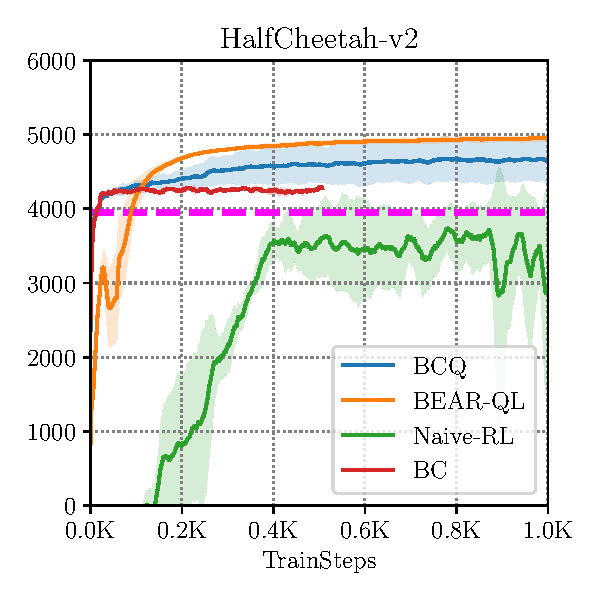
\includegraphics[width=0.99\linewidth]{chapters/bear/images/cheetah_mediocre.pdf}
%     \end{subfigure}
%     \begin{subfigure}[t]{0.23\textwidth}
%         \centering
%         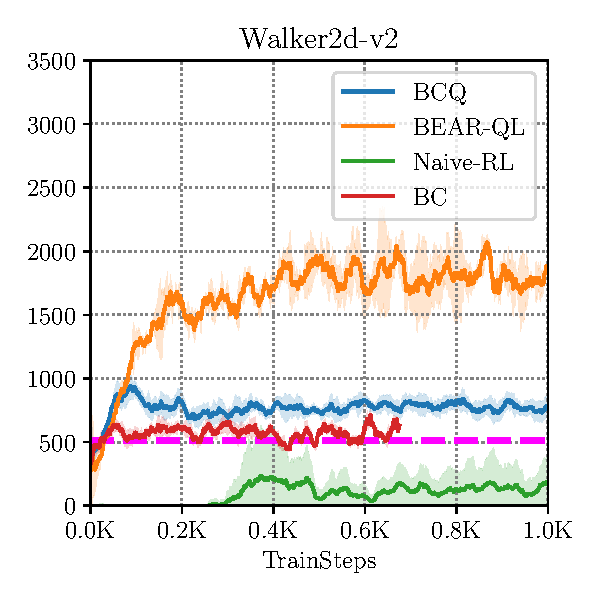
\includegraphics[width=0.99\linewidth]{chapters/bear/images/walker_mediocre_final_again.pdf}
%         % \caption{}
%     \end{subfigure}
%     ~
%     \begin{subfigure}[t]{0.23\textwidth}
%         \centering
%         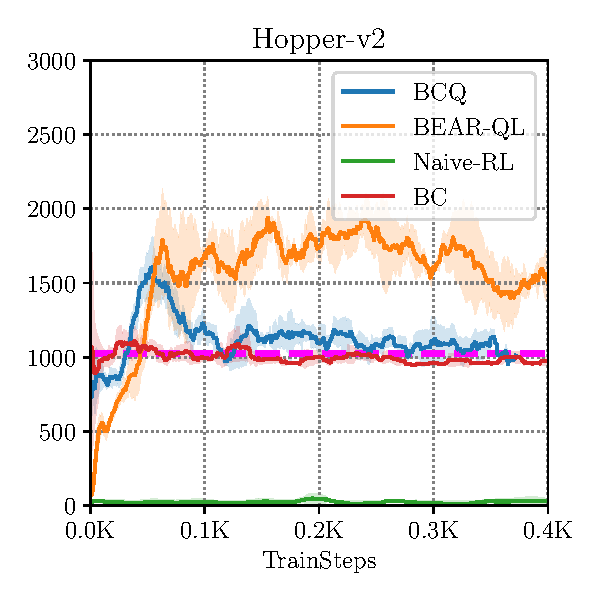
\includegraphics[width=0.99\linewidth]{chapters/bear/images/hopper_mediocre_final_new.pdf}
%         % \caption{}
%     \end{subfigure}
%     ~
%     \begin{subfigure}[t]{0.23\textwidth}
%         \centering
%         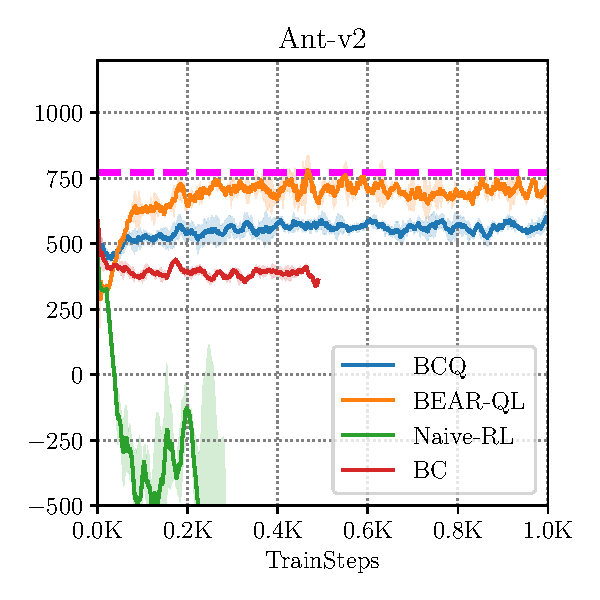
\includegraphics[width=0.99\linewidth]{chapters/bear/images/ant_mediocre_final.pdf}
%         % \caption{}
%     \end{subfigure}
%     \caption{ \footnotesize Average performance of BEAR, BCQ, Na\"ive RL and BC on medium-quality data averaged over 5 seeds. BEAR outperforms both BCQ and Na\"ive RL. Average return over the training data is indicated by the magenta line. One step on the x-axis corresponds to 1000 gradient steps.}
%     \label{fig:mediocre}
%     \vspace{-0.1in}
% \end{figure*}

% \vspace{-5pt}
\subsection{Performance on Random and Optimal Datasets}
In Figure~\ref{fig:optimal_random}, we show the performance of each method when trained on data from a random policy (top) and a near-optimal policy (bottom). In both cases, our method BEAR achieves good results, consistently exceeding the average dataset return on random data, and matching the optimal policy return on optimal data. Na\"{i}ve RL also often does well on random data. For a random data policy, all actions are in-distribution, since they all have equal probability. This is consistent with our hypothesis that OOD actions are one of the main sources of error in off-policy learning on static datasets. The prior BCQ method~\cite{fujimoto2018off} performs well on optimal data but performs poorly on random data, where the constraint is too strict. These results show that BEAR is more robust to the dataset composition, and can learn consistently in a variety of settings. We find that KL-control and DQfD can be unstable in these settings.  

{Finally, in Figure \ref{fig:humanoid}, we  show that BEAR outperforms other considered prior methods in the challenging Humanoid-v2 environment as well, in two cases -- Medium-quality data and random data.}

\begin{figure}
        \centering
        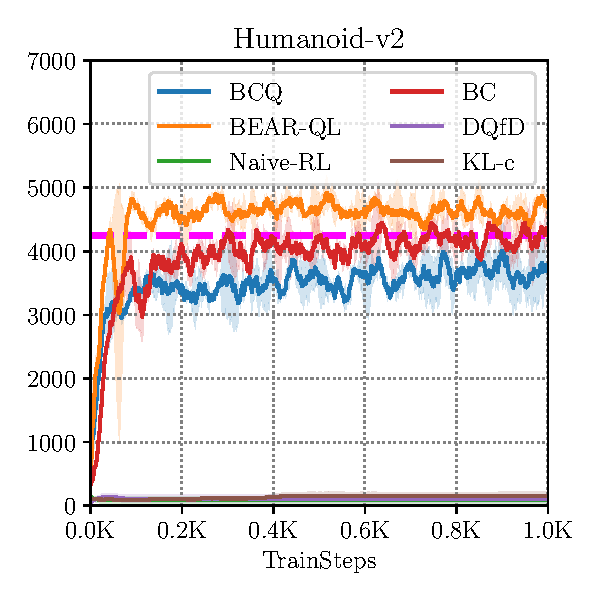
\includegraphics[width=0.4\linewidth]{chapters/bear/images/images_camera_ready/humanoid_mediocre_camera_ready.pdf}
       ~
        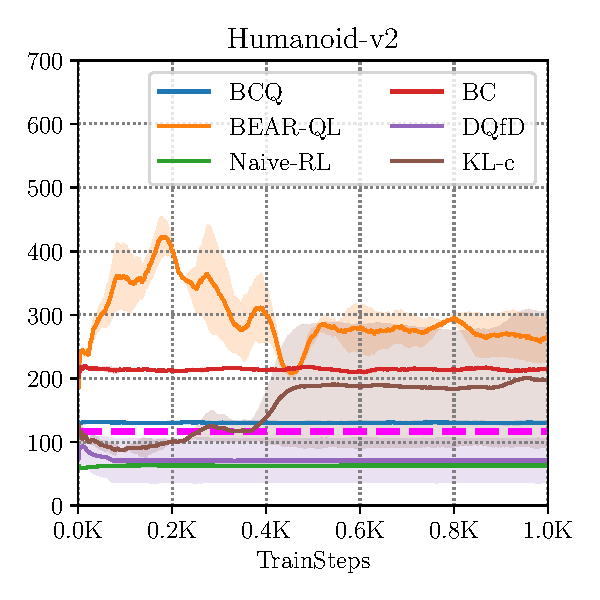
\includegraphics[width=0.4\linewidth]{chapters/bear/images/images_camera_ready/humanoid_random_camera_ready.pdf}
      \caption{\label{fig:humanoid} \footnotesize Performance of BEAR, BCQ, Na\"ive RL and BC on medium-quality (left) and random (right) data in the Humanoid-v2 environment. Note that BEAR outperforms prior methods.}
\end{figure}

%With random data, BCQ is expected to not perform well, as it constrains actions to the actions seen in the dataset at a particular state. On the other hand, a na\"ive off-policy RL algorithm is expected to perform well in these settings. In Figure~\ref{fig:optimal_random}, we show that BEAR outperforms \cite{fujimoto2018off} drastically while still performing comparable to the na\"ive RL algorithm in HalfCheetah-v2, and Hopper-v2, and outperforming it on Walker2d-v2 and Ant-v2 tasks. On optimal data, as the suboptimality bias is small, the best solution is to imitate the behavior policy. BEAR learns to imitate the behavior policy, and maintains stably there. In this setting, na\"ive-RL algorithm fails to learn (and mostly converges to the minimum possible reward, that can be obtained in the environment). Overall, BEAR is robust to the dataset composition, and can consistently perform in all settings -- mediocre, random and optimal data. Figure~\ref{fig:optimal_random} summarizes the average evaluation return of the learned policy as a function of training steps.

% show that DQNs are empirically less stable than off-policy actor critic algorithms(TD3). In all cases, note that BCQ~\cite{fujimoto18addressing} often ends up imitating the baseline, which explains the reason for poor performance on random data, and fast convergence to optimal performance on optimal data. However, the versatility of BEAR demonstrates its use as a practical algorithm irrespective of the quality of the dataset $\dataset$. We also examine the amount of deviation from the true MC-returns of the actor and the learned estimate of the Q-value, which again suggests that BEAR can learn reliable estimates of Q-values without excessive overestimation as observed in TD3, while achieving better expected return performance over BCQ. \TODO{Q vs MC figure left}

\begin{figure}
    \centering
    \begin{subfigure}[t]{0.23\textwidth}
        \centering
        % 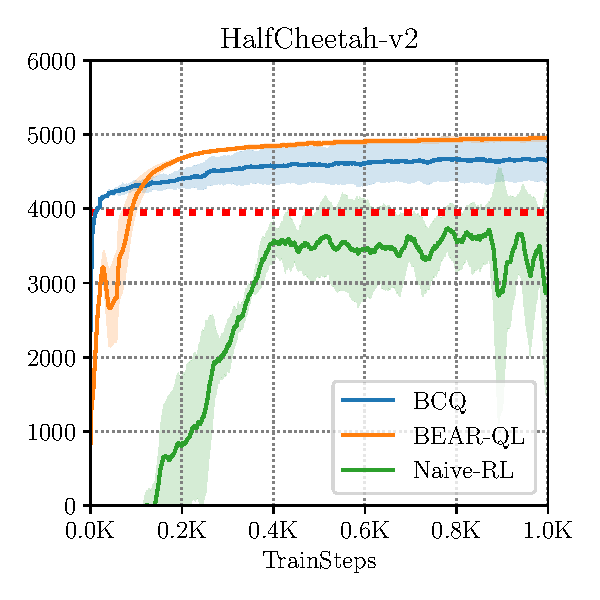
\includegraphics[width=0.99\linewidth]{chapters/bear/images/cheetah_mediocre_final.pdf}
        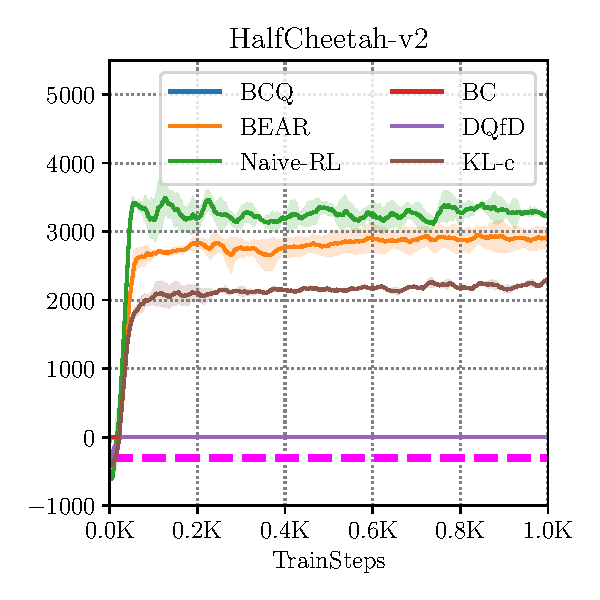
\includegraphics[width=0.99\linewidth]{chapters/bear/images/images_camera_ready/cheetah_random_final_camera_ready.pdf}
        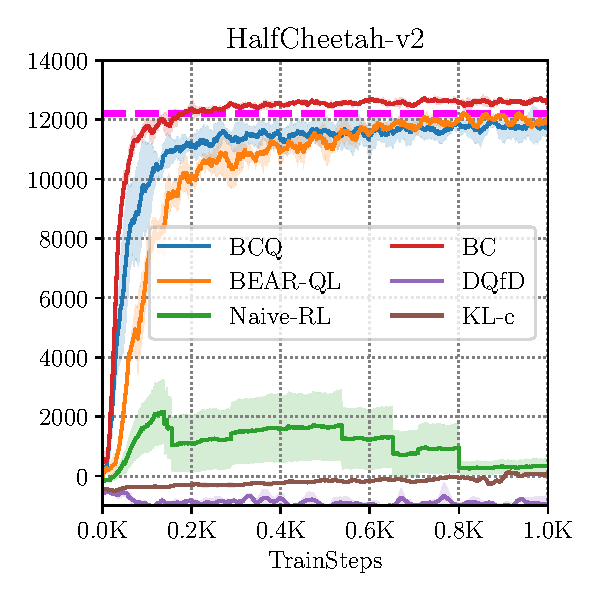
\includegraphics[width=0.99\linewidth]{chapters/bear/images/images_camera_ready/cheetah_optimal_camera_ready_new.pdf}
        % \caption{}
    \end{subfigure}%
    ~ 
    \begin{subfigure}[t]{0.23\textwidth}
        \centering
        % 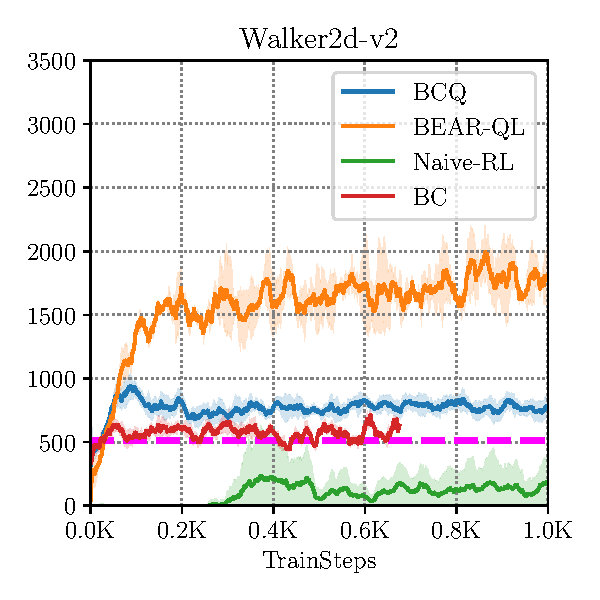
\includegraphics[width=0.99\linewidth]{chapters/bear/images/walker_mediocre_final.pdf}
        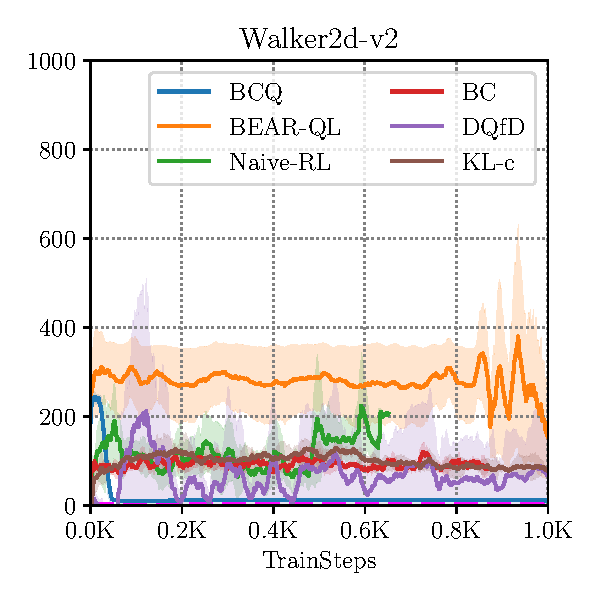
\includegraphics[width=0.99\linewidth]{chapters/bear/images/images_camera_ready/walker_random_camera_ready.pdf}
        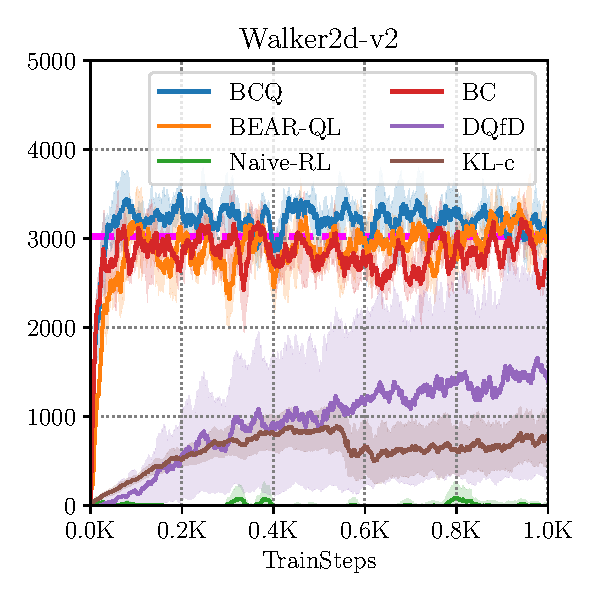
\includegraphics[width=0.99\linewidth]{chapters/bear/images/images_camera_ready/walker_optimal_camera_ready.pdf}
        % \caption{}
    \end{subfigure}
    ~
    \begin{subfigure}[t]{0.23\textwidth}
        \centering
        % 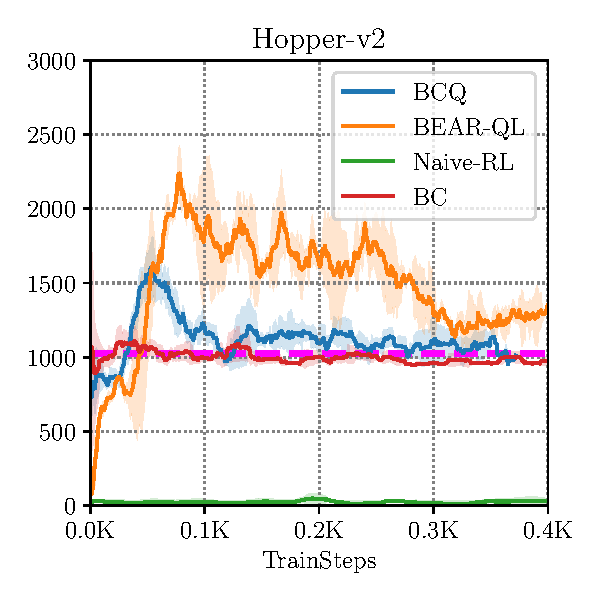
\includegraphics[width=0.99\linewidth]{chapters/bear/images/hopper_mediocre_final.pdf}
        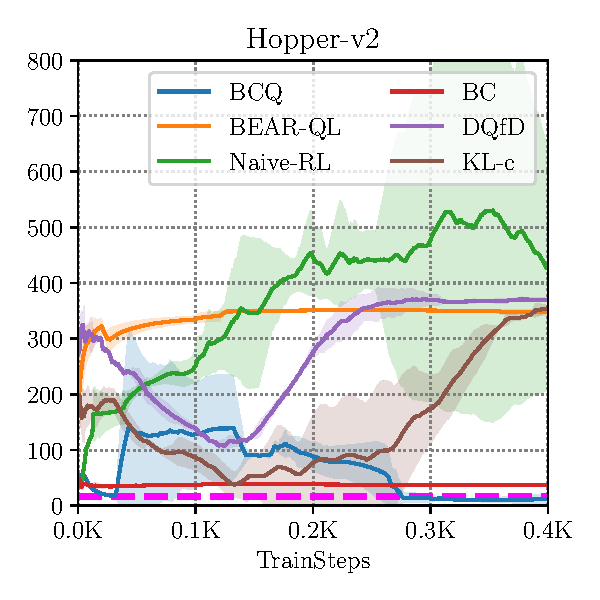
\includegraphics[width=0.99\linewidth]{chapters/bear/images/images_camera_ready/hopper_random_camera_ready.pdf}
        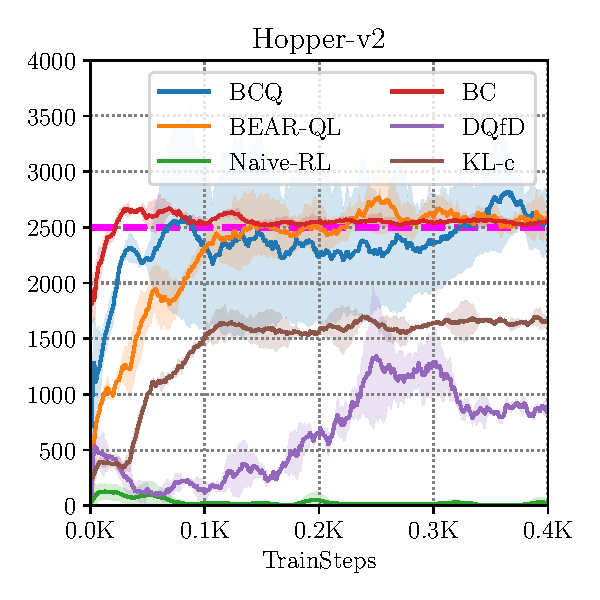
\includegraphics[width=0.99\linewidth]{chapters/bear/images/images_camera_ready/hopper_optimal_camera_ready.pdf}
        % \caption{}
    \end{subfigure}
    ~
    \begin{subfigure}[t]{0.23\textwidth}
        \centering
        % 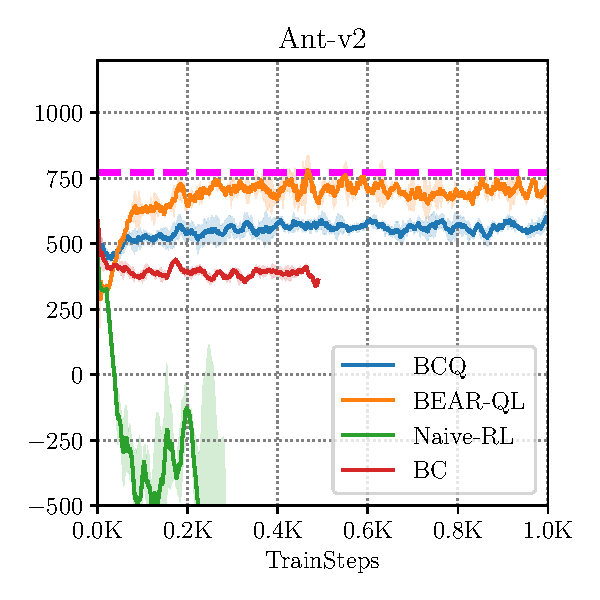
\includegraphics[width=0.99\linewidth]{chapters/bear/images/ant_mediocre_final.pdf}
        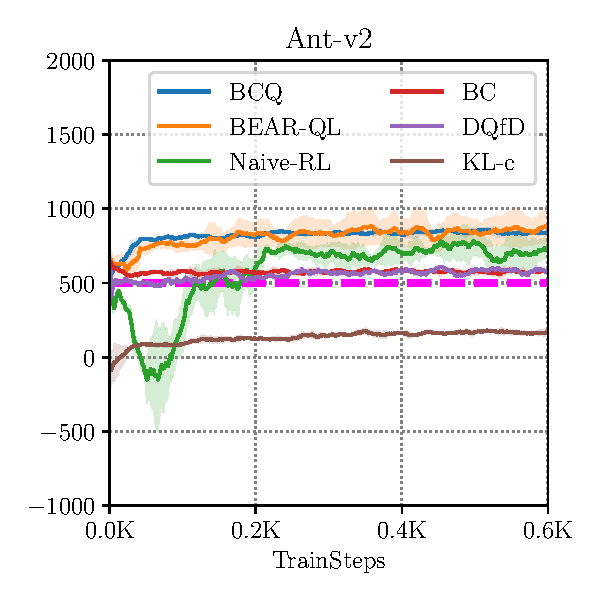
\includegraphics[width=0.99\linewidth]{chapters/bear/images/images_camera_ready/ant_random_camera_ready.pdf}
        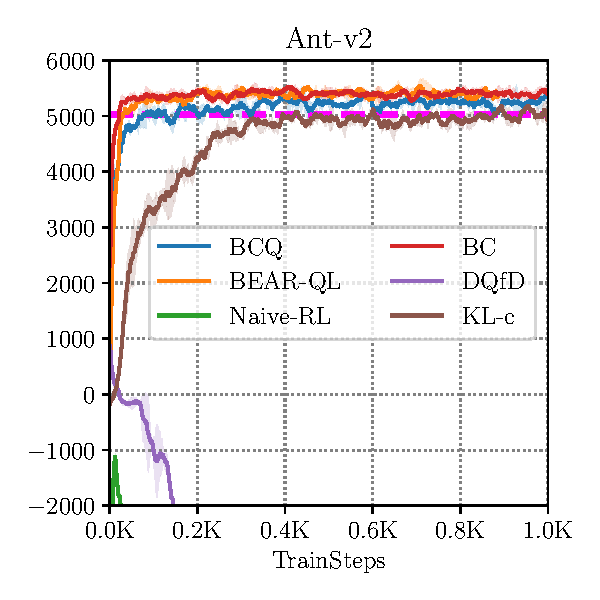
\includegraphics[width=0.99\linewidth]{chapters/bear/images/images_camera_ready/ant_optimal_camera_ready.pdf}
        % \caption{}
    \end{subfigure}
    \caption{\label{fig:optimal_random} \footnotesize Average performance of BEAR, BCQ, Na\"ive RL and BC on random data (top row) and optimal data (bottom row) over 5 seeds. BEAR is the only algorithm capable of learning in both scenarios. Na\"{i}ve RL cannot handle optimal data, since it does not illustrate mistakes, and BCQ favors a behavioral cloning strategy (performs quite close to behavior cloning in most cases), causing it to fail on random data. Average return over the training dataset is indicated by the dashed magenta line.}
\end{figure}

% \begin{figure*}[t!]
% \vspace{-0.1in}
%     \centering
%     \begin{subfigure}[t]{0.23\textwidth}
%         \centering
%         % 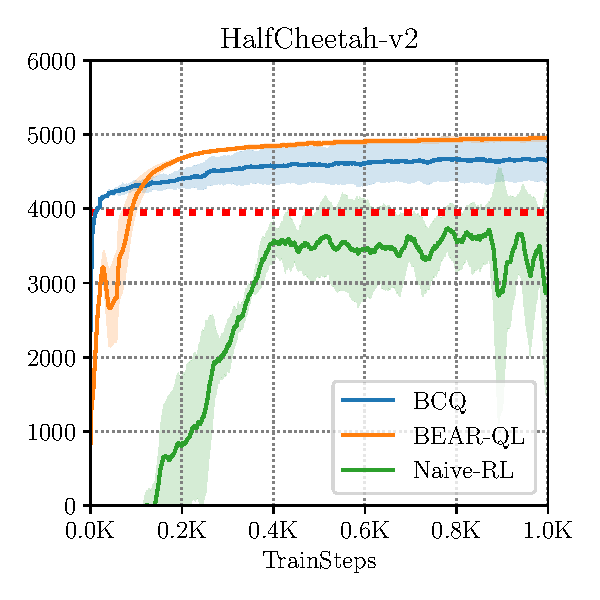
\includegraphics[width=0.99\linewidth]{chapters/bear/images/cheetah_mediocre_final.pdf}
%         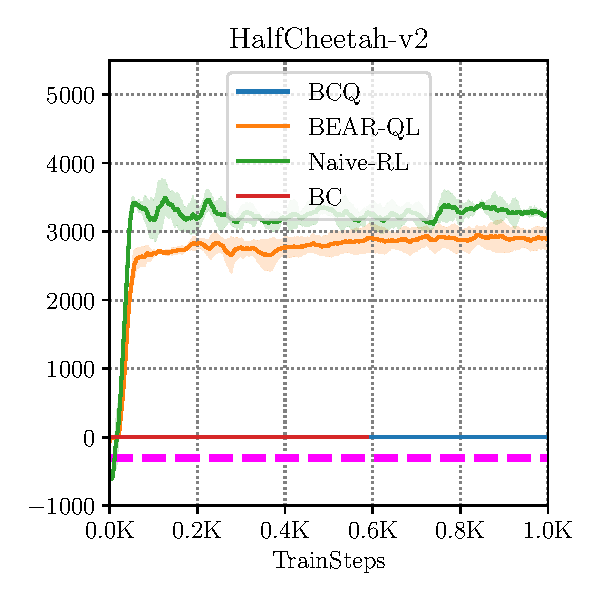
\includegraphics[width=0.99\linewidth]{chapters/bear/images/cheetah_random_final.pdf}
%         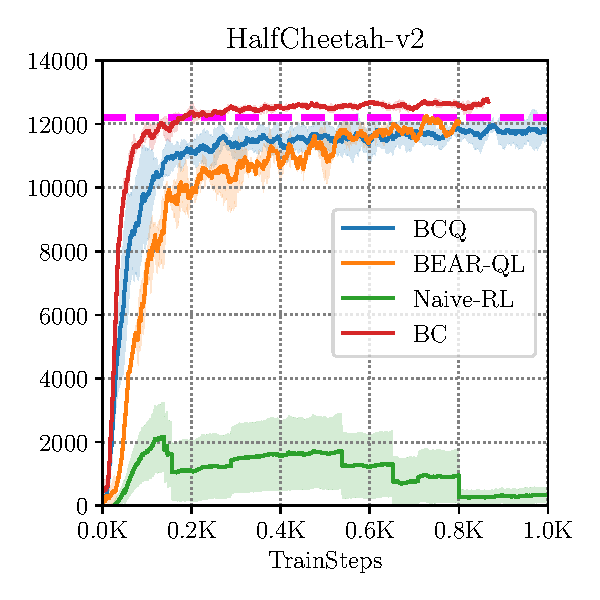
\includegraphics[width=0.99\linewidth]{chapters/bear/images/cheetah_optimal_final.pdf}
%         % \caption{}
%     \end{subfigure}%
%     ~ 
%     \begin{subfigure}[t]{0.23\textwidth}
%         \centering
%         % 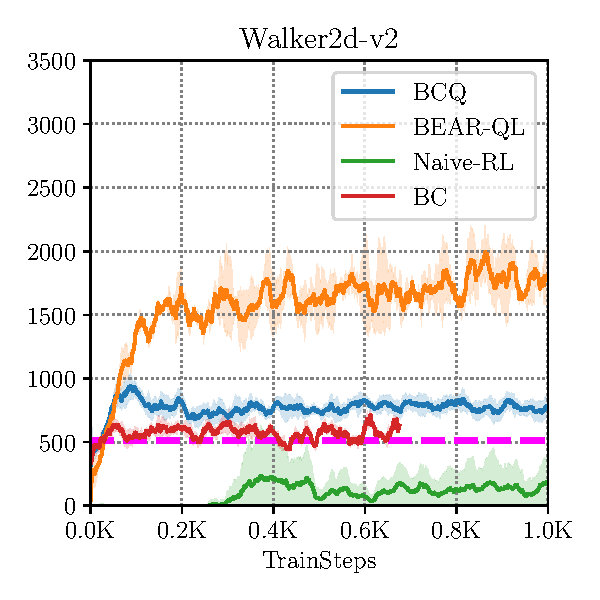
\includegraphics[width=0.99\linewidth]{chapters/bear/images/walker_mediocre_final.pdf}
%         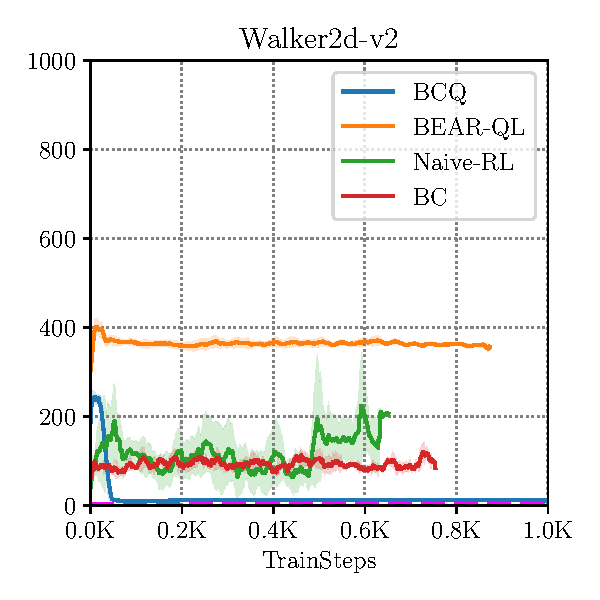
\includegraphics[width=0.99\linewidth]{chapters/bear/images/walker_random_final.pdf}
%         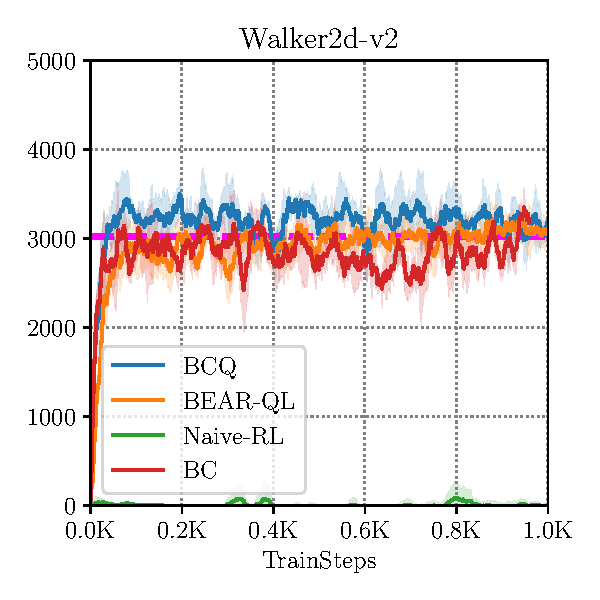
\includegraphics[width=0.99\linewidth]{chapters/bear/images/walker_optimal_final.pdf}
%         % \caption{}
%     \end{subfigure}
%     ~
%     \begin{subfigure}[t]{0.23\textwidth}
%         \centering
%         % 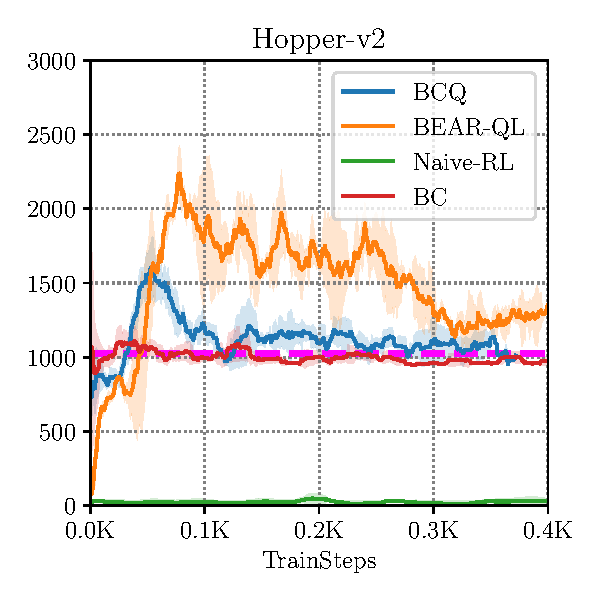
\includegraphics[width=0.99\linewidth]{chapters/bear/images/hopper_mediocre_final.pdf}
%         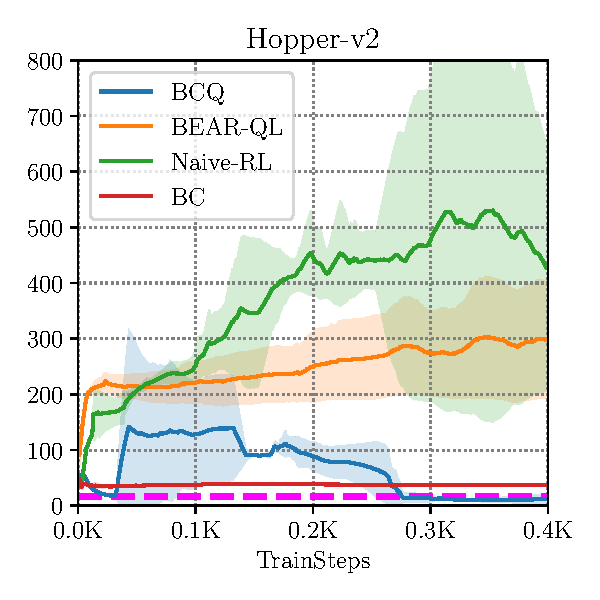
\includegraphics[width=0.99\linewidth]{chapters/bear/images/hopper_random_final.pdf}
%         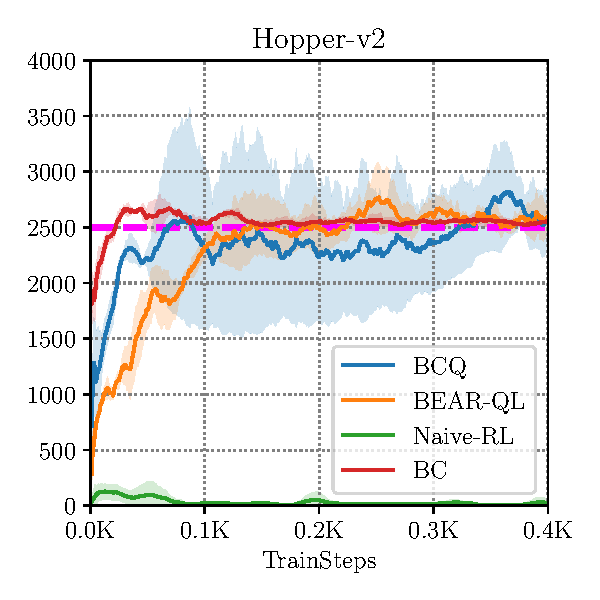
\includegraphics[width=0.99\linewidth]{chapters/bear/images/hopper_optimal_final.pdf}
%         % \caption{}
%     \end{subfigure}
%     ~
%     \begin{subfigure}[t]{0.23\textwidth}
%         \centering
%         % 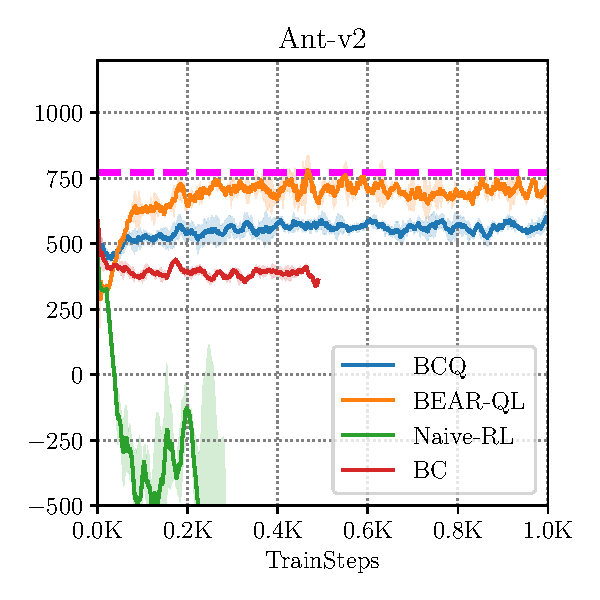
\includegraphics[width=0.99\linewidth]{chapters/bear/images/ant_mediocre_final.pdf}
%         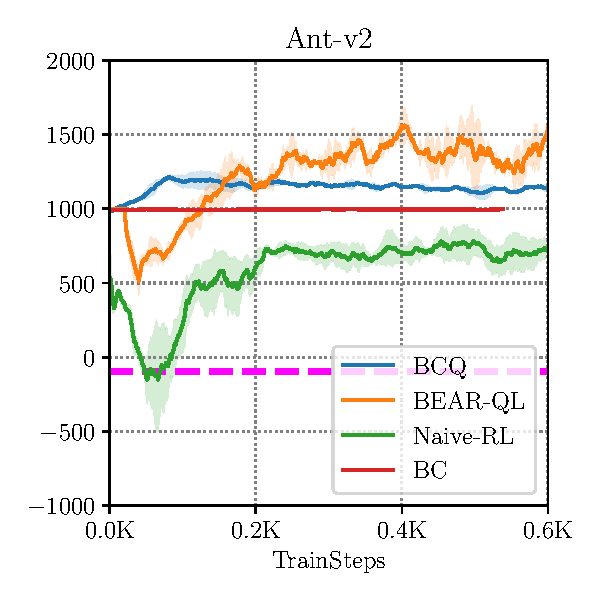
\includegraphics[width=0.99\linewidth]{chapters/bear/images/ant_random_final.pdf}
%         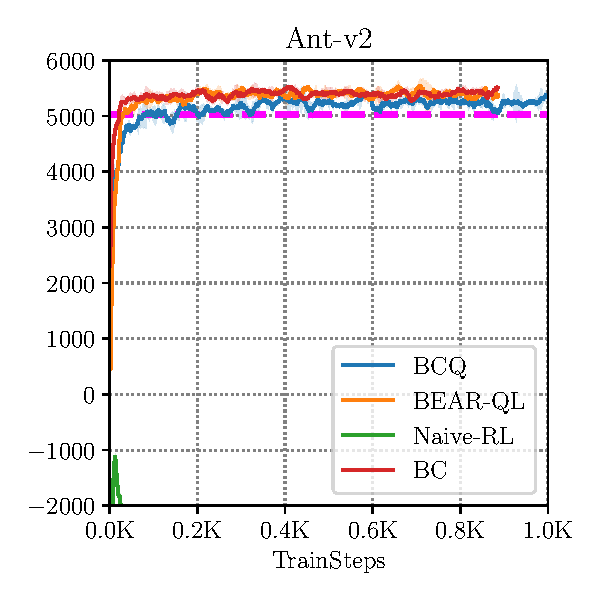
\includegraphics[width=0.99\linewidth]{chapters/bear/images/ant_optimal_final.pdf}
%         % \caption{}
%     \end{subfigure}
%     \caption{\footnotesize Average performance of BEAR, BCQ, Na\"ive RL and BC on random data (top row) and optimal data (bottom row) over 5 seeds. BEAR is the only algorithm capable of learning in both scenarios. Na\"{i}ve RL cannot handle optimal data, since it does not illustrate mistakes, and BCQ favors a behavioral cloning strategy (performs quite close to behavior cloning in most cases), causing it to fail on random data. Average return over the training dataset is indicated by the dashed magenta line.}
%     \label{fig:optimal_random}
%     \vspace{-0.1in}
% \end{figure*}

% \begin{figure*}[t!]
%     \centering
%     \begin{subfigure}[t]{0.31\textwidth}
%         \centering
%         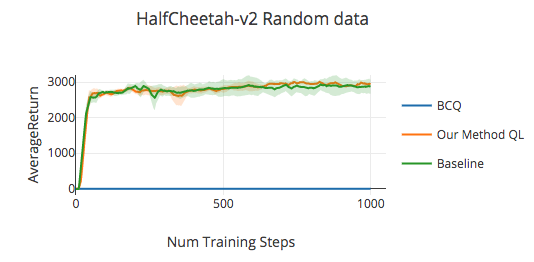
\includegraphics[width=0.99\linewidth]{chapters/bear/images/random_halfcheetah.png}
%         \caption{ }
%     \end{subfigure}%
%     ~ 
%     \begin{subfigure}[t]{0.31\textwidth}
%         \centering
%         \includegraphics[width=0.99\linewidth]{chapters/bear/images/mediocre_walker.png}
%         \caption{ }
%     \end{subfigure}
%     ~
%     \begin{subfigure}[t]{0.31\textwidth}
%         \centering
%         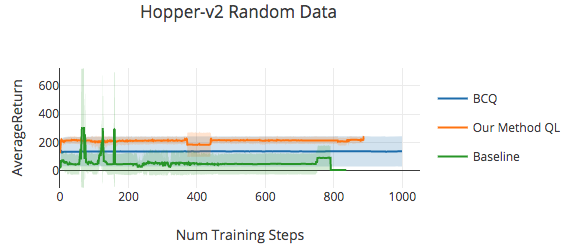
\includegraphics[width=0.99\linewidth]{chapters/bear/images/random_hopper.png}
%         \caption{ }
%     \end{subfigure}
%     \caption{Random Data}
% \end{figure*}

% \begin{figure*}[t!]
%     \centering
%     \begin{subfigure}[t]{0.23\textwidth}
%         \centering
%         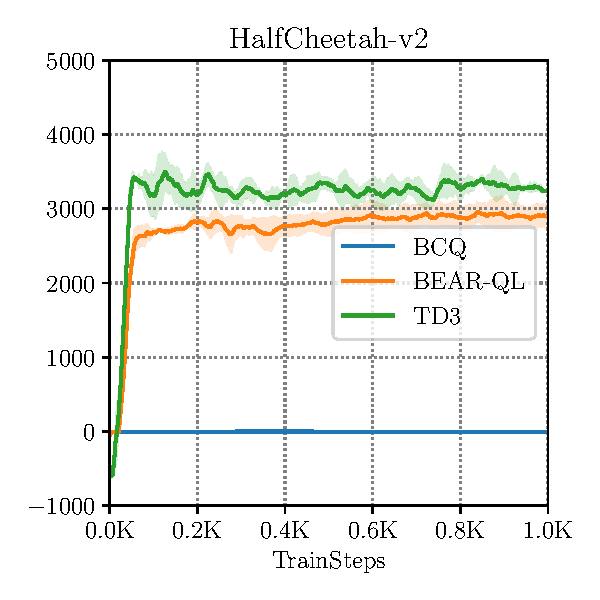
\includegraphics[width=0.99\linewidth]{chapters/bear/images/cheetah_random.pdf}
%         \caption{ }
%     \end{subfigure}%
%     ~ 
%     \begin{subfigure}[t]{0.23\textwidth}
%         \centering
%         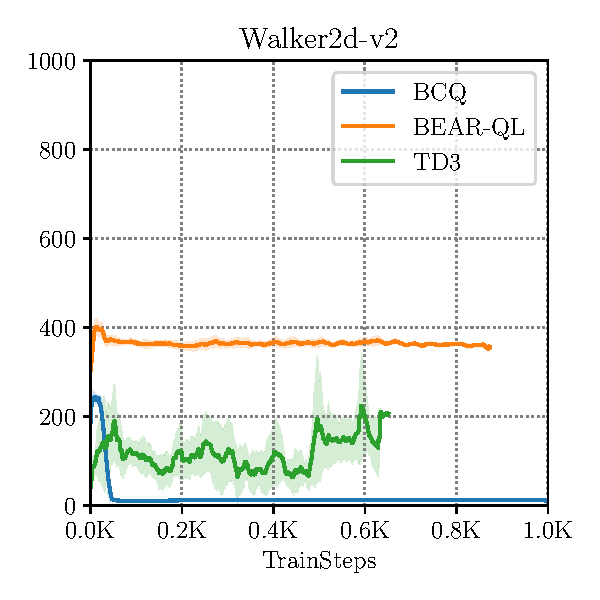
\includegraphics[width=0.99\linewidth]{chapters/bear/images/walker_random.pdf}
%         \caption{ }
%     \end{subfigure}
%     ~
%     \begin{subfigure}[t]{0.23\textwidth}
%         \centering
%         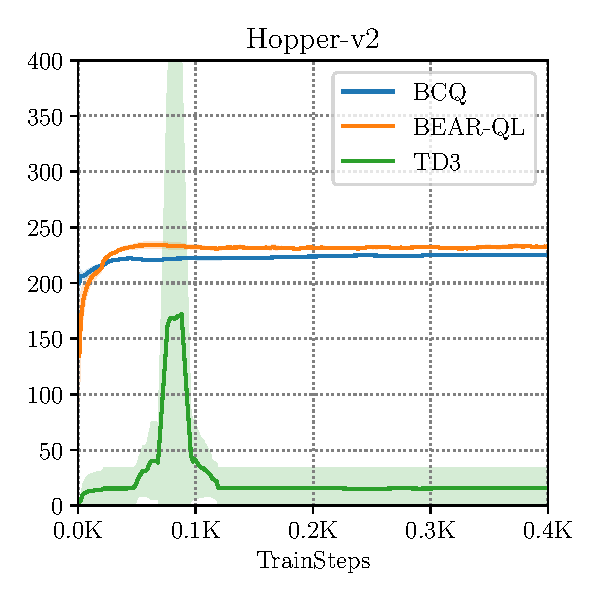
\includegraphics[width=0.99\linewidth]{chapters/bear/images/hopper_random.pdf}
%         \caption{ }
%     \end{subfigure}
%     ~
%     \begin{subfigure}[t]{0.23\textwidth}
%         \centering
%         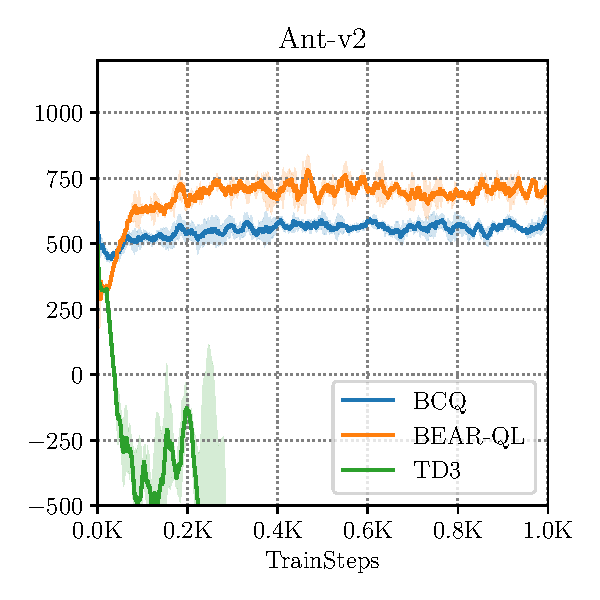
\includegraphics[width=0.99\linewidth]{chapters/bear/images/ant_mediocre.pdf}
%         \caption{ }
%     \end{subfigure}
%     \caption{Random Data}
% \end{figure*}

% \begin{figure*}[t!]
%     \centering
%     \begin{subfigure}[t]{0.23\textwidth}
%         \centering
%         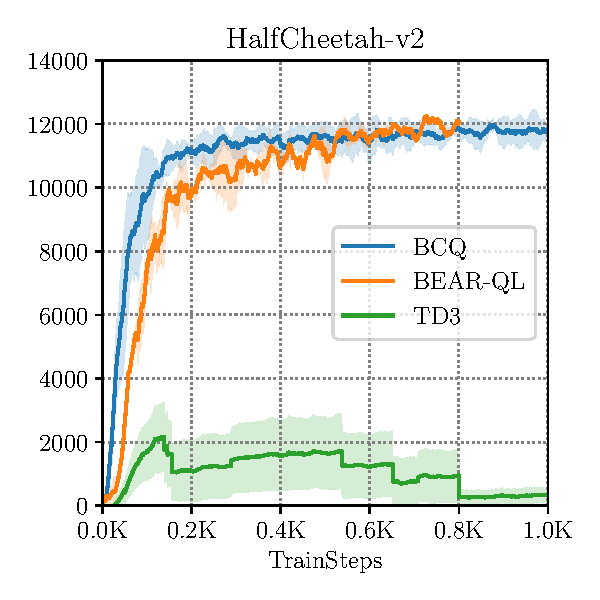
\includegraphics[width=0.99\linewidth]{chapters/bear/images/cheetah_optimal.pdf}
%         \caption{ }
%     \end{subfigure}%
%     ~ 
%     \begin{subfigure}[t]{0.23\textwidth}
%         \centering
%         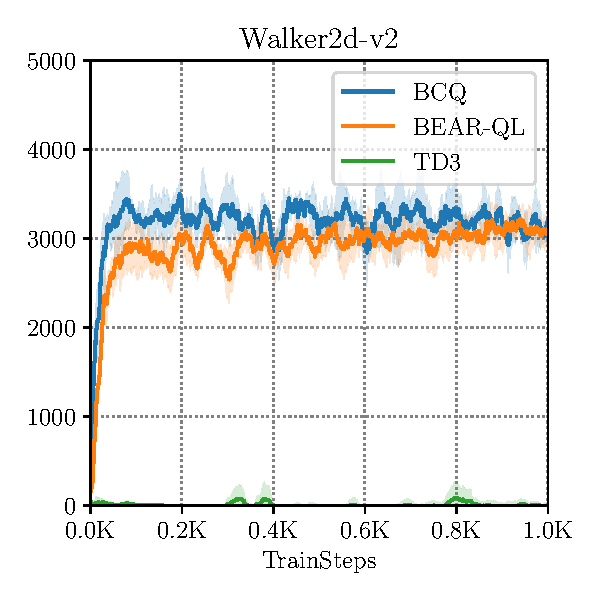
\includegraphics[width=0.99\linewidth]{chapters/bear/images/walker_optimal.pdf}
%         \caption{ }
%     \end{subfigure}
%     ~
%     \begin{subfigure}[t]{0.23\textwidth}
%         \centering
%         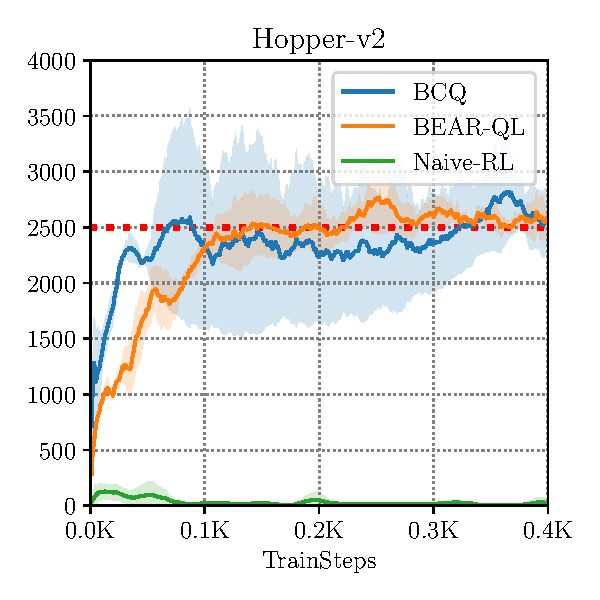
\includegraphics[width=0.99\linewidth]{chapters/bear/images/hopper_optimal.pdf}
%         \caption{ }
%     \end{subfigure}
%     ~
%     \begin{subfigure}[t]{0.23\textwidth}
%         \centering
%         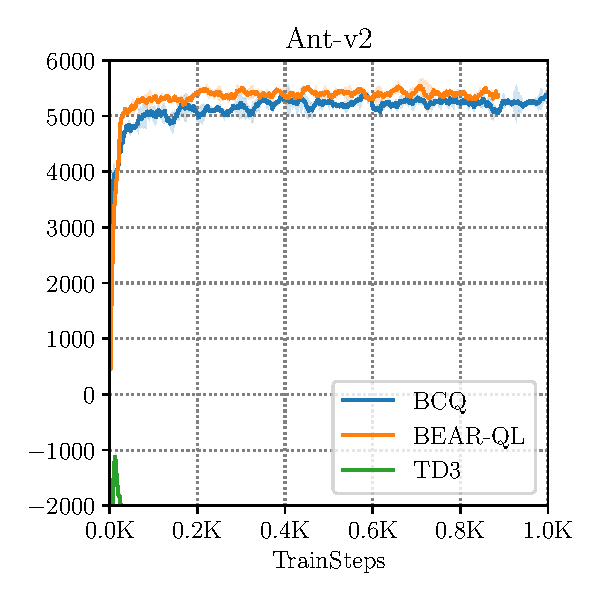
\includegraphics[width=0.99\linewidth]{chapters/bear/images/ant_optimal.pdf}
%         \caption{ }
%     \end{subfigure}
%     \caption{Optimal Data}
% \end{figure*}

\iffalse

\vspace{-5pt}
\subsection{Analysis of BEAR}
\label{subsec:ablations}
In this section, we aim to analyze different components of our method via an ablation study. Our first ablation studies the support constraint discussed in Section~\ref{sec:bear}, which uses MMD to measure support. We replace it with a more standard KL-divergence distribution constraint, which measures similarity in density. 
% \TODO{how is this done if we don't have the behavior policy? do you assume access for this study? -- we train a behavior policy on the data and then constrain to that with KL or MMD (so it should be a fair comparison)}
Our hypothesis is that this should provide a more conservative constraint, since matching distributions is not necessary for matching support. KL-divergence performs well in some cases, such as with optimal data, but as shown in Figure~\ref{fig:ablations}, it performs worse than MMD on medium-quality data. Even when KL-divergence is hand tuned fully, so as to prevent instability issues it still performs worse than a not-well tuned MMD constraint. We provide the results for this setting in the Appendix. We also vary the number of samples $n$ that are used to compute the MMD constraint. We find that smaller n ($\approx$ 4 or 5) gives better performance. Although the difference is not large, consistently better performance with 4 samples leans in favour of our hypothesis that an intermediate number of samples works well for support matching, and hence is less restrictive.

\fi
% Next, we study whether using a conservative Q-value estimate by subtracting the variance in the ensemble helps with learning. As shown in Figure~\ref{fig:ablations}, the conservative estimate 
%  makes a comparatively smaller difference than the use of MMD, providing some benefit on one task, while somewhat hurting performance on another.
% The ensemble produces more conservative estimates, which can result in underestimation in practice, and prevent overestimation divergence.

%The third factor in the ablation study is whether the usage of conservative estimates of Q-values subtracting the variance of the $Q$-ensemble helps. We find that on Hopper, usage of ensembles helps, whereas on Walker2d using ensembles hurts as the algorithm tends to underestimate Q-values. Figure~\ref{subfig:ensembles_ablation} demonstrates the average trend on 2 environments -- Hopper and Walker.




% \subsection{Generalization performance on datasets collected using a mixture of markovian policies.}
% We finally test our BEAR method in the case where the dataset $\dataset$ cannot be generated by a \TODO{Sergey and George: What's your opinion on having this section about non-markovian policies? This was one reason why Fujimoto got rejected. {https://openreview.net/forum?id=S1zlmnA5K7\&noteId=HJeQ-p0F2Q} }
% \TODO{Exp List: - Ant multiple + Point Mass multiple
%                 - with BCQ, BEAR, BEAR with n=1, BEAR without ensemble}

% \begin{figure}
%     \centering
%     \includegraphics{}
%     \caption{Caption}
%     \label{fig:my_label}
% \end{figure}
% \section{Discussion and Future Work}
\vspace{-5pt}
The goal in our work was to study off-policy reinforcement learning with static datasets. We theoretically and empirically analyze how error propagates in off-policy RL due to the use of out-of-distribution actions for computing the target values in the Bellman backup. Our experiments suggest that this source of error is one of the primary issues afflicting off-policy RL: increasing the number of samples does not appear to mitigate the degradation issue (Figure~\ref{fig:divergence}), and training with na\"{i}ve RL on data from a random policy, where there are no out-of-distribution actions, shows much less degradation than training on data from more focused policies (Figure~\ref{fig:optimal_random}). Armed with this insight, we develop a method for mitigating the effect of out-of-distribution actions, which we call BEAR-QL. BEAR-QL constrains the backup to use actions that have non-negligible support under the data distribution, but without being overly conservative in constraining the learned policy. We observe experimentally that BEAR-QL achieves good performance across a range of tasks, and across a range of dataset compositions, learning well on random, medium-quality, and expert data.

% \vspace{-0.15in}
\begin{wrapfigure}{r}{0.51\textwidth}
        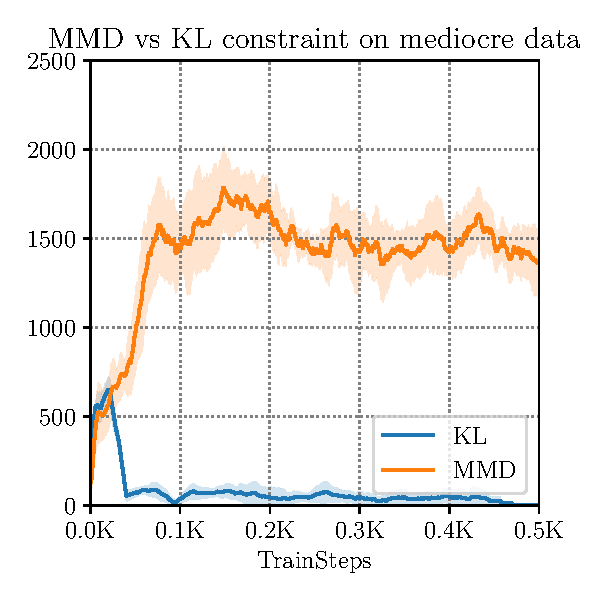
\includegraphics[width=0.48\linewidth]{chapters/bear/images/kl_vs_mmd_ablation_final.pdf}
       ~
        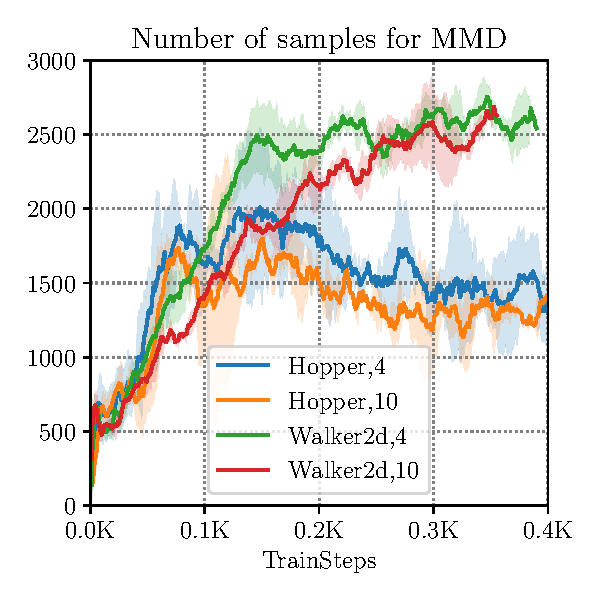
\includegraphics[width=0.48\linewidth]{chapters/bear/images/num_samples_ablation.pdf}
        % ~
        % \includegraphics[width=0.31\linewidth]{images/ensembles_ablation_final.pdf}
      \caption{\footnotesize Average return (averaged Hopper-v2 and Walker2d-v2) as a function of train steps for ablation studies from Section~\ref{subsec:ablations}. (a) MMD constrained optimization is more stable and leads to better returns, (b) 4 sample MMD is more performant than 10.}
    %   and (c) Ensemble variance has mixed benefit.}
      \label{fig:ablations}
\vspace{-10pt}
\end{wrapfigure}

While BEAR-QL substantially stabilizes off-policy RL, we believe that this problem merits further study. One limitation of our current method is that, although the learned policies are more performant than those acquired with na\"{i}ve RL, performance sometimes still tends to degrade for long learning runs. An exciting direction for future work would be to develop an early stopping condition for RL, perhaps by generalizing the notion of validation error to reinforcement learning. {A limitation of approaches that perform constrained-action selection is that they can be overly conservative when compared to methods that constrain state-distributions directly, especially with datasets collected from mixtures of policies. We leave it to future work to design algorithms that can directly constrain state distributions. A theoretically robust method for support matching efficiently in high-dimensional continuous action spaces is a question for future research. Perhaps methods from outside RL, predominantly used in domain adaptation, such as using asymmetric f-divergences~\citep{wu19domain} can be used for support restriction.} Another promising future direction is to examine how well BEAR-QL can work on large-scale off-policy learning problems, of the sort that are likely to arise in domains such as robotics, autonomous driving, operations research, and commerce. If RL algorithms can learn effectively from large-scale off-policy datasets, reinforcement learning can become a truly data-driven discipline, benefiting from the same advantage in generalization that has been seen in recent years in supervised learning fields, where large datasets have enabled rapid progress in terms of accuracy and generalization~\cite{imagenet_cvpr09}.

\section*{Acknowledgements}
We thank Kristian Hartikainen for sharing implementations of RL algorithms and for help in debugging certain issues. We thank Matthew Soh for help in setting up environments. We thank Aurick Zhou, Chelsea Finn, Abhishek Gupta, Kelvin Xu and Rishabh Agarwal for informative discussions. We thank Ofir Nachum for comments on an earlier draft of this paper. We thank Google, NVIDIA, and Amazon for providing computational resources. This research was supported by Berkeley DeepDrive, JPMorgan Chase \& Co., NSF IIS-1651843 and IIS-1614653, the DARPA Assured Autonomy program, and ARL DCIST CRA W911NF-17-2-0181.

\vspace{-0.4cm}
\begin{AIbox}{\large{\textbf{Abstract}}}
\vspace{4mm}
In this chapter, we utilize offline RL to the problem of designing hardware accelerators, i.e., chips that are tailored towards improving the efficiency of running certain software applications. For instance, TPU accelerators aim to optimize the performance of machine learning models. While a paradigm shift towards specializing hardware is already starting to show promising results, designers still need to spend considerable manual effort and perform large number of time-consuming simulations to find accelerators that can accelerate multiple target applications while obeying design constraints. Moreover, a designer would need to typically start from scratch every time the set of target applications or design constraints change in such a ``simulation-driven'' workflow. An alternative paradigm is to use an offline approach that utilizes logged simulation data, to architect hardware accelerators, without needing active simulations. This is different from supervised learning: instead of predicting a performance metric associated with an accelerator, we wish to find a new accelerator that attains  near-optimal metrics, much in the same way where we wish to find a near-optimal policy in offline RL. In this problem, our offline RL based approach, dubbed \primemethodname, not only alleviates the need to run time-consuming simulation, but also enables data reuse and applies even when set of target applications changes.
% Our approach learns a conservative estimate of the desired reward function, utilizes infeasible points and optimizes the design against this estimate without any additional simulator queries during optimization.
\primemethodname\ architects accelerators for both single and multiple applications, improving performance upon state-of-the-art simulation-driven methods by about 1.54$\times$ and 1.20$\times$, while reducing the total simulation time by 93\% and 99\%, respectively.
% In addition, \primemethodname\ architects accelerators for unseen applications in a zero-shot setting, outperforming simulation-based methods by 1.26$\times$.
\vspace{2mm}
\end{AIbox}


\section{Introduction}
\label{sec:intro}
%% motivation, brief description of the problem statement
The death of Moore's Law~\citep{esmaeilzadeh2011dark} and its spiraling effect on the semiconductor industry have driven the growth of specialized hardware accelerators. These specialized accelerators are tailored to specific applications~\citep{yazdanbakhsh2021apollo,reagen2017case,prac_dse:mascots:2019,shi2020learned}. To design specialized accelerators, designers first spend considerable amounts of time developing simulators that closely model the real accelerator performance, and then optimize the accelerator using the simulator. While such simulators can automate accelerator design, this requires a large number of simulator queries for each new design, both in terms of simulation time and compute requirements, and this cost increases with the size of the design space~\citep{yazdanbakhsh2021evaluation,shi2020learned,hegdemind}.
%
Moreover, most of the accelerators in the design space are typically infeasible~\citep{hegdemind,yazdanbakhsh2021apollo} because of build errors in silicon or compilation/mapping failures. 
%
When the target applications change or a new application is added, the complete simulation-driven procedure is generally repeated.
%
To make such approaches efficient and practically viable, designers typically ``bake-in'' constraints or otherwise narrow the search space, but such constraints can leave out high-performing solutions~\citep{dmazerunner,timeloop,marvel}.

%% Transition to the new paradigm, define data-driven stuff, etc
An alternate approach, proposed in this work, is to devise a \textit{data-driven} optimization method that only utilizes a database of previously tested accelerator designs, annotated with measured performance metrics, to produce new optimized designs \emph{without} additional active queries to an explicit silicon or a cycle-accurate simulator.
%
Such a data-driven approach provides three key benefits: \textbf{(1)} it significantly shortens the recurring cost of running large-scale simulation sweeps, \textbf{(2)} it alleviates the need to explicitly bake in domain knowledge or search space pruning, and {\textbf{(3)} it enables data re-use by empowering the designer to optimize accelerators for new unseen applications, by the virtue of effective generalization.}
%
While data-driven approaches have shown promising results in biology~\citep{fu2021offline,brookes19a,trabucco2021conservative},
using offline optimization methods to design accelerators 
has been challenging primarily due to the abundance of infeasible design points~\citep{yazdanbakhsh2021apollo,hegdemind}.

%% The key idea of our method
The key contribution of this paper is a data-driven approach, \primemethodname\,, to automatically architect high-performing application-specific accelerators by using only previously collected offline data.
%
\primemethodname\ learns a robust surrogate model of the task objective function from an existing offline dataset, and finds high-performing application-specific accelerators by optimizing the architectural parameters against this learned surrogate function, as shown in Figure~\ref{fig:overview}. While na\"ively learned
%
\begin{figure}[t!]
    \centering
    \vspace{-0.1cm}
    \includegraphics[width=0.8\linewidth]{chapters/prime/figs/overview/prime-overview.pdf}
    \vspace{-0.2cm}
    \caption{\footnotesize{\textbf{Overview of \primemethodname.} We use a one-time collected dataset of prior accelerator designs, including TPU-style~\citep{yazdanbakhsh2021evaluation}, NVDLA-style~\citep{nvdla}, and ShiDianNao-style~\citep{shidiannao} accelerators to train a conservative surrogate model, which is used to design accelerators to meet desired goals and constraints.}}
    \vspace{-0.4cm}
    \label{fig:overview}
\end{figure}
surrogate functions usually produces poor-performing, out-of-distribution designs that appear quite optimistic under the learned surrogate~\citep{kumar2019model,brookes19a,trabucco2021conservative}.
%
The robust surrogate in \primemethodname\ is explicitly trained to prevent overestimation on ``adversarial'' designs that would be found during optimization.
%
Furthermore, in contrast to prior works that discard infeasible points~\citep{hegdemind,trabucco2021conservative}, our proposed method instead incorporates infeasible points when learning the conservative surrogate by treating them as additional negative samples.
%
During evaluation, \primemethodname\ optimizes the learned conservative surrogate.

Our results show that \primemethodname\ architects hardware accelerators that improve over the best design in the training dataset, on average, by 2.46$\times$ (up to 6.7$\times$) when specializing for a single application. 
%
In this case, \primemethodname\ also improves over the best conventional simulator-driven optimization methods by 1.54$\times$ (up to 6.6$\times$).
%
These performance improvements are obtained while reducing the total simulation time to merely 7\% and 1\% of that of the simulator-driven methods for single-task and multi-task optimization, respectively.
%
More importantly, a contextual version of \primemethodname\ can design accelerators that are \emph{jointly optimal} for a set of \textit{nine} applications without requiring any additional domain information.
%
In this challenging setting, \primemethodname\ improves over simulator-driven methods, which tend to scale poorly as more applications are added, by 1.38$\times$.
%
Finally, we show that the surrogates trained with \primemethodname\ on a set of training applications can be readily used to obtain accelerators for \textit{unseen} target applications, without any retraining on the new application.
%
Even in this \emph{zero-shot} optimization scenario, \primemethodname\ outperforms simulator-based methods that require re-training and active simulation queries by up to 1.67$\times$.
%
In summary, \primemethodname\ allows us to effectively address the shortcomings of simulation-driven approaches, it: (1) significantly reduces the simulation time, (2) enables data reuse and enjoys generalization properties, and (3) does not require domain-specific engineering or search space pruning.
%

\vspace{-0.1cm}
\section{Background on Hardware Accelerators}
\vspace{-0.1cm}
\label{sec:background}
The goal of specialized hardware accelerators---Google TPUs~\citep{jouppi2017datacenter,edgetpu:arxiv:2020}, Nvidia GPUs~\citep{nvidia}, GraphCore~\citep{graphcore}---is to improve the performance of specific applications, such as machine learning models. To design such accelerators, architects typically create a parameterized design and sweep over parameters using simulation.

\niparagraph{Target hardware accelerators.}
%
Our primary evaluation uses an industry-grade and highly parameterized template-based accelerator following prior work~\citep{yazdanbakhsh2021evaluation}.
%
This template enables architects to determine the organization of various components, such as compute units, memory cells, memory, etc., by searching for these configurations in a discrete design space. Some ML applications may have large memory requirements (e.g., large language models~\citep{brown2020language}) demanding sufficient on-chip memory resources, while others may benefit from more compute blocks. The hardware design workflow directly selects the values of these parameters.
%
In addition to this accelerator and to further show the generality of our method to other accelerator design problems, we evaluate two distinct dataflow accelerators with different search spaces, namely NVDLA-style~\citep{nvdla} and ShiDianNao-style~\citep{shidiannao} from~\citet{kao2020confuciux} (See Section~\ref{sec:eval} and Appendix~\ref{sec:dla_shi_fast} for a detailed discussion; See Table~\ref{table:dla_shi} for results).

\begin{wrapfigure}{r}{0.4\textwidth}
    \centering
    \vspace{-0.1in}
    \includegraphics[width=0.98\linewidth]{chapters/prime/figs/accelerator/template-accel.png}
    \caption{An industry-level machine learning accelerator~\cite{yazdanbakhsh2021evaluation}.}
    \label{fig:template_accel}
    \vspace{-0.4cm}
    \label{fig:accels}
\end{wrapfigure} 

\niparagraph{How does an accelerator work?}
%
We briefly explain the computation flow on our template-based accelerators (Figure~\ref{fig:template_accel}) and refer the readers to Appendix~\ref{sec:dla_shi_fast} for details on other accelerators.
%
This template-based accelerator is a 2D array of processing elements (PEs). Each PE is capable of performing matrix multiplications in a single instruction multiple data (SIMD) paradigm~\citep{simd}. A controller orchestrates the data transfer (both activations and model parameters) between off-chip DRAM memory and the on-chip buffers and also reads in and manages the instructions (e.g. convolution, pooling, etc.) for execution. The computation stages on such accelerators start by sending a set of activations to the compute lanes, executing them in SIMD manner, and either storing the partial computation results or offloading them back into off-chip memory.
%
Compared to prior works~\citep{hegdemind,shidiannao,kao2020confuciux}, this parameterization is unique---it includes multiple compute lanes per each PE and enables SIMD execution model within each compute lane---and yields a distinct accelerator search space accompanied by an end-to-end simulation framework. More details in Appendix~\ref{sec:dla_shi_fast}.
%

\vspace{-0.2cm}
\section{Problem Statement, Training Data and Evaluation Protocol}
\label{sec:accel}
\vspace{-0.2cm}
%
Our template-based parameterization maps the accelerator, denoted as $\rvx$, to a discrete design space, $\rvx = [\rvx_1, \rvx_2, \cdots, \rvx_K]$, and each $\rvx_i$ is a discrete-valued variable representing one component of the microarchitectural template, as shown in Table~\ref{tab:arch_params} (See Appendix~\ref{sec:dla_shi_fast} for the description of other accelerator search spaces studied in our work). In our context, the accelerator $\rvx$ plays the same role as an action $\mathbf{a}$.

%
An accelerator design maybe be infeasible due to various reasons, such as a compilation failure or the limitations of physical implementation, and we denote the set of all such feasibility criterion as $\mathrm{Feasible}(\rvx)$. The feasibility criterion depends on both the target software and the underlying hardware, and it is not easy to identify if a given $\rvx$ is infeasible without running explicit simulation. We will require our design procedure to not only learn the value of the objective function but also to learn to navigate through infeasible solutions to performant feasible solutions $\rvx^*$ satisfying $\mathrm{Feasible}(\rvx^*) = 1$. 

Our training dataset $\mathcal{D}$ consists of a modest set of accelerators $\rvx_i$ that are randomly sampled from the design space and evaluated by the hardware simulator. We partition the dataset $\mathcal{D}$ into two subsets, $\mathcal{D}_\text{feasible}$ and $\mathcal{D}_\text{infeasible}$. Let $f(\rvx)$ denote the desired objective (e.g., latency, power, etc.) we intend to optimize over the space of accelerators $\rvx$. We do not possess functional access to $f(\rvx)$, and the optimizer can only access $f(\rvx)$ values for accelerators $\rvx$ in the feasible partition of the data, $\mathcal{D}_\text{feasible}$.
%
For all infeasible accelerators, the simulator does not provide any value of $f(\rvx)$.
In addition to satisfying feasibility, the optimizer must handle explicit constraints on parameters such as area and power~\citep{flynn2011computer}. In our applications, we impose an explicit area constraint, $\mathrm{Area}(\rvx) \leq \review{\alpha_0}$, though additional explicit constraints are also possible. 
%
To account for different constraints, we formulate this task as a constrained optimization problem.
%
Formally:  
\begin{equation}
\label{eqn:opt_prob}
\vspace{-0.2cm}
\begin{aligned}
\min_{\rvx}~ & f(\rvx)
~~~\textrm{s.t.}~~~\mathrm{Area}(\rvx) \leq \review{\alpha_0}, ~~~ \mathrm{Feasible}(\rvx) = 1 \\
\quad &~\text{on}~~ \mathcal{D} = \mathcal{D}_\text{feasible} \cup \mathcal{D}_\text{infeasible} = \{(\rvx_1, \rvy_1), \cdots, (\rvx_N, \rvy_N)\} \cup \{\rvx'_1, \cdots, \rvx'_{N'}\}
\end{aligned}
\end{equation}

While Equation~\ref{eqn:opt_prob} may appear similar to a typical black-box optimization problem, solving it over the space of accelerator designs is challenging due to the large number of infeasible points, the need to handle explicit design constraints, and the difficulty in navigating the non-smooth landscape (See Figure~\ref{fig:ds_dist_all} and Figure~\ref{fig:appx_ds} in the Appendix) of the objective function.
%


\begin{table*}[t!]
\small
\centering
% \vspace*{0.1cm}
\caption{The accelerator design space parameters for the primary accelerator search space targeted in this work. The maximum possible number of accelerator designs (including feasible and infeasible designs) is 452,760,000. \methodname\ only uses a small randomly sampled subset of the search space.}
\label{tab:arch_params}
\vspace{-0.1cm}
\resizebox{0.8\textwidth}{!}{\begin{tabular}{l|l||l|l}
\toprule
\textbf{Accelerator Parameter} &\textbf{\# Discrete Values} & \textbf{Accelerator Parameter} & \textbf{\# Discrete Values}\\\midrule
\# of PEs-X & 10 & \# of PEs-Y & 10\\\hline
PE Memory & 7 & \# of Cores & 7\\\hline
Core Memory & 11 & \# of Compute Lanes & 10\\\hline
Instruction Memory & 4 & Parameter Memory & 5\\\hline
Activation Memory & 7 & DRAM Bandwidth & 6\\
\bottomrule
\end{tabular}}
\vspace{-0.2cm}
\end{table*}

\niparagraph{What makes optimization over accelerators challenging?} Compared to other domains where model-based optimization methods have been applied~\citep{brookes19a,trabucco2021conservative}, optimizing accelerators introduces a number of practical challenges.
%
First, accelerator design spaces typically feature a narrow manifold of feasible accelerators within a sea of infeasible points~\citep{prac_dse:mascots:2019,shi2020learned,gelbart2014bayesian}, as visualized in Figure~\ref{fig:ds_dist_all} and Appendix (Figure~\ref{fig:tsne_infeasible}).
%
While some of these infeasible points can be identified via simple rules (e.g. estimating chip area usage), most infeasible points correspond to failures during compilation or hardware simulation. These infeasible points are generally not straightforward to formulate into the optimization problem and requires simulation~\citep{shi2020learned,timeloop,yazdanbakhsh2021apollo}.

Second, the optimization objective can exhibit high sensitivity to small variations in some architecture parameters (Figure~\ref{fig:appx_ds_memory}) in some regions of the design space, but remain relatively insensitive in other parts, resulting in a complex optimization landscape. This suggests that optimization algorithms based on local parameter updates (e.g., gradient ascent,  evolutionary schemes, etc.) may have a challenging task traversing the nearly flat landscape of the objective, which can lead to poor performance.
\begin{figure}[t]
    \begin{center}
    \begin{minipage}{\linewidth}
    \centering
    \includegraphics[width=0.35\linewidth]{chapters/prime/figs/dataset/dist.pdf}
    \vspace{-0.1cm}
    \label{fig:ds_dist}
    \centering
    \includegraphics[width=0.35\linewidth]{chapters/prime/figs/dataset/dist_large.pdf}
    \label{fig:ds_dist_large}
    \end{minipage}
    \end{center}
    \vspace{-0.2cm}
    \caption{\footnotesize{\textbf{Left:} histogram of infeasible (right orange bar with large score values) and feasible (left cluster of bars) data points for MobileNetEdgeTPU; \textbf{Right:} zoomed-in histogram (different number of bins) focused on feasible points highlighting the variable latencies.}}
    \vspace{-0.2cm}
    \label{fig:ds_dist_all}
\end{figure}

\niparagraph{Training dataset.}
%
We used an offline dataset $\mathcal{D}$ of (accelerator parameters, latency) via random sampling from the space of 452M possible accelerator configurations.
%
Our method is only provided with a relatively modest set of feasible points ($\leq 8000$ points) for training, and these points are the \emph{worst-performing} feasible points across the pool of randomly sampled data.
%
This dataset is meant to reflect an easily obtainable and an application-agnostic dataset of accelerators that could have been generated once and stored to disk, or might come from real physical experiments. 
%
We emphasize that no assumptions or domain knowledge about the application use case was made during dataset collection.
%
Table~\ref{tab:models} depicts the list of target applications, evaluated in this work, includes three variations of MobileNet~\citep{edgetpu:arxiv:2020,mnv2:arxiv:2018,mnv3:cvpr:2019}, three in-house industry-level models for object detection (M4, M5, M6; names redacted to prevent anonymity violation), a U-net model~\citep{unet}, and two RNN-based encoder-decoder language models~\citep{trnn01,trnn02,trnn03,trnn04}. 
%
These applications span the gamut from small models, such as \msix, with only 0.4~MB model parameters that demands less on-chip memory, to the medium-sized models ($\geq$~5~MB), such as MobileNetV3 and \mfour models, and large models ($\geq$~19~MB), such as t-RNNs, hence requiring larger on-chip memory. 
%
\begin{table*}[h]
\vspace{0.05cm}
\small{
\centering
% \vspace*{0.1cm}
\caption{\footnotesize Description of applications, their domains, number of (convolutions, depth-wise convolutions, feed-forward) XLA ops, model parameter size, instruction sizes in bytes, number of compute operations.}
\label{tab:models}
\vspace{-0.1cm}
\resizebox{\textwidth}{!}{\begin{tabular}{l|l|c|r|r|r}
\toprule
\textbf{Name}&\textbf{Domain}&\textbf{\# of XLA Ops (Conv, D/W, FF)}&\textbf{Model Param}&\textbf{Instr. Size}&\textbf{\# of Compute Ops.}\\\midrule
{\textbf{MobileNetEdgeTPU}} &Image Class.&(45, 13, 1)&3.87~MB&476,736&1,989,811,168\\\hline
{\textbf{MobileNetV2}}&Image Class.&(35, 17, 1)&3.31~MB&416,032&609,353,376\\\hline
{\textbf{MobileNetV3}}&Image Class.&(32, 15, 17)&5.20~MB&1,331,360&449,219,600\\\hline
\textbf{\mfour}&Object Det.&(32, 13, 2)&6.23~MB&317,600&3,471,920,128\\\hline
\textbf{\mfive}&Object Det.&(47, 27, 0)&2.16~MB&328,672&939,752,960\\\hline
\textbf{\msix}&Object Det.&(53, 33, 2)&0.41~MB&369,952&228,146,848\\\hline
\textbf{U-Net}&Image Seg.&(35, 0, 0)&3.69~MB&224,992&13,707,214,848\\\hline
\textbf{t-RNN Dec}&Speech Rec.&(0, 0, 19)&19~MB&915,008&40,116,224\\\hline
\textbf{t-RNN Enc}&Speech Rec.&(0, 0, 18)&21.62~MB&909,696&45,621,248\\
\bottomrule
\end{tabular}}
}
\vspace{-0.25cm}
\end{table*}

\niparagraph{Evaluation protocol.}
%
To compare simulator-driven methods and our data-driven method, we limit the number of feasible points (costly to evaluate) that can be used by any algorithm to equal amounts. We still provide infeasible points to any method and leave it up to the optimization method to use it or not.
This ensures our comparisons are fair in terms of the amount of data available to each method.
However, it is worthwhile to note that in contrast to our method where \emph{worse-quality} data points from small offline dataset are used, the simulator-driven methods have an inherent advantage because they can steer the query process towards the points that are more likely to be better in terms of performance.
Following prior work in data-driven design~\citep{brookes19a}, we evaluate each run of a method by first sampling the top $n=256$ design candidates according to the algorithm's predictions, evaluating all of these under the ground truth objective function and recording the performance of the best accelerator design. The final reported results is the median of ground truth objective values across five independent runs.

\section{\primemethodname: Architecting Accelerators via Conservative Models}
\label{sec:method}
%
As shown in Figure~\ref{fig:method}, our method first learns a conservative surrogate model of the optimization objective using the offline dataset. Then, it optimizes this learned model using a discrete optimizer. The optimization process does not require access to a simulator, nor to real-world experiments beyond the initial dataset, except when evaluating the final top-performing $n=256$ designs (Section~\ref{sec:accel}). This is built on the principle of conservative value estimation for offline RL from Chapter ??: while conservative value estimation methods attempt to estimate a pessimistic value-function, we can consider our approach as a special case involving a single decision-making step.

\begin{figure}
    \centering
    \vspace{-0.3cm}
    \includegraphics[width=0.7\linewidth]{chapters/prime/figs/overview/mbo-method.pdf}
    \vspace{-0.1cm}
    \caption{\small{Overview of \primemethodname\ which trains a conservative model ${f}_\theta(\rvx_i)$ using Equation~\ref{eqn:final_training}. Our neural net model for ${f}_\theta(\rvx)$ utilizes two transformer layers~\citep{vaswani2017attention}, and a multi-headed architecture which is pooled via a soft-attention layer.}}
    \vspace{-0.3cm}
    \label{fig:method}
\end{figure}

\subsection{Learning Conservative Models Using Logged Offline Data}
Our goal is to utilize a logged dataset of feasible accelerator designs labeled with the desired performance metric (e.g., latency),  $\mathcal{D}_\text{feasible}$, and additional infeasible designs, $\mathcal{D}_\text{infeasible}$ to learn a mapping ${f}_\theta: \mathcal{X} \rightarrow \mathbb{R}$, that maps the accelerator configuration $\rvx$ to its corresponding metric $y$. This learned conservative model can then be optimized by the optimizer. While a straightforward approach for learning such a mapping is to train it via supervised regression (which is equivalent to standard temporal-difference learning for value estimation when considering one-step decision-making scenarios), by minimizing the mean-squared error $\E_{\rvx_i, y_i \sim \mathcal{D}}[(f_\theta(\rvx_i) - y_i)^2]$, as we have seen in this dissertation and in other prior works~\citep{kumar2019model}, such predictive models can arbitrarily overestimate the value of an unseen input $\rvx_i$. This can cause the optimizer to find a solution $\rvx^*$ that performs poorly in the simulator but looks promising under the learned model. We empirically validate this overestimation hypothesis and find it to confound the optimizer in on our problem domain as well (See Figure~\ref{fig:cali_plot} in Appendix). 

To prevent overestimated values at unseen inputs from confounding the optimizer, we follow the conservative value estimation recipe from Chapter ?? (specifically, Equation ??) and train $f_\theta(\rvx)$ with an additional term that explicitly maximizes the function value $f_\theta(\rvx)$ at out-of-distribution $\rvx$ values. Note that instead of minimizing the value $f_\theta(\rvx)$ on unseen $\rvx$, we maximize this value because the problem in Equation ?? requires us to find the minimum of the ground-truth function. Such unseen designs $\rvx$ are ``negative mined'' by running a few iterations of a stochastic optimization procedure that aims to maximize $f_\theta$ in the inner loop. In the context of this single-step decision-making problem, this procedure is analogous to adversarial training~\citep{goodfellow2014explaining}. Equation~\ref{eqn:training} formalizes this objective:
\newcommand{\editcolor}{black}
\begin{equation}
\label{eqn:training}
    \theta^* := \arg \min_\theta~~ \mathcal{L}(\theta):= \E_{\rvx_i, y_i \sim \mathcal{D}_{\text{feasible}}} \left[ (f_\theta(\rvx_i) - y_i)^2 \right] - \alpha \E_{\rvx^{-}_i \sim \textcolor{\editcolor}{\mathrm{Opt}(f_\theta)}} \left[f_\theta(\rvx^-_i) \right].
\end{equation}
$\rvx^{-}_i$ denotes the negative samples produced from an optimizer $\mathrm{Opt}(\cdot)$ that attempts to maximize the current learned objective model, $f_\theta$. We will discuss our choice of $\mathrm{Opt}$ in the Appendix Section~\ref{app:details}.  
 
\subsection{Incorporating Design Constraints by Training on Infeasible Points}
While conservative value estimation methods simply discuss how we can optimize Equation~\ref{eqn:training} by learning a conservative model, this is not enough when optimizing over accelerators, as we will also show empirically (Appendix~\ref{app:additional_experiments}).
This is because explicitly minimizing for out-of-distribution designs does not provide any information about accelerator design constraints. Fortunately, this information can be provided by infeasible points, $\mathcal{D}_\text{infeasible}$. The training procedure in Equation~\ref{eqn:training} provides a simple way to do incorporate such infeasible points: we simply incorporate $\rvx'_i \sim \mathcal{D}_{\text{infeasible}}$ as additional out-of-distribution samples and maximize the prediction at these points.
This gives rise to our final objective:
\begin{equation}
\label{eqn:final_training}
    \min_\theta~~ \mathcal{L}^\text{inf}(\theta) := \mathcal{L}(\theta)
    - \textcolor{blue}{\beta \E_{\rvx'_i \sim \mathcal{D}_{\text{infeasible}}}\left[ f_\theta(\rvx'_i) \right]}
\end{equation}

\subsection{Optimizing Multiple Applications and Zero-Shot Design}
%
One of the central benefits of an offline learning approach is that it enables learning powerful models that generalize over the space of applications, potentially being effective for new unseen application domains. In our experiments, we evaluate \primemethodname\ on designing accelerators for multiple applications denoted as $k=1, \cdots, K$, jointly or for a novel unseen application. In this case, we utilized a dataset $\mathcal{D} = \{\mathcal{D}_1, \cdots, \mathcal{D}_K\}$, where each $\mathcal{D}_k$ consists of a set of accelerator designs, annotated with the latency value and the feasibility criterion for a given application $k$. While there are a few overlapping designs in different parts of the dataset annotated for different applications, most of the designs only appear in one part. To train a single conservative model $f_\theta(\cdot)$ for multiple applications, we extend the training procedure in Equation~\ref{eqn:final_training} to incorporate \textit{context vectors} $\rvc_k \in \mathbb{R}^d$ for various applications driven by a list of application properties in Table~\ref{tab:models}. A context vector is akin to a state in the context of full sequential reinforcement learning. 

The learned function in this setting is now conditioned on the context $f_\theta(\rvx, \rvc_k)$. We train $f_\theta$ via the objective in Equation~\ref{eqn:final_training}, but in expectation over all the contexts and their corresponding datasets: $\min_\theta \E_{\textcolor{blue}{k \sim [K]}}\left[\mathcal{L}^\text{inf}_k(\theta)\right]$. Once such a contextual model is learned, we can either optimize the average models across a set of contexts $\{\rvc_i, \rvc_2, \cdots, \rvc_n\}$ to obtain an accelerator that is optimal for multiple applications simultaneously on an average (``multi-model'' optimization), or optimize this contextual model for a novel context vector, corresponding to an unseen application (``zero-shot'' generalization). In this case, \primemethodname\ is not allowed to train on any data corresponding to this new unseen application.  While such zero-shot generalization might appear surprising at first, note that the context vectors are not simply one-hot vectors, but consist of parameters with semantic information, which the conservative model can generalize over.

~

\niparagraph{Learned conservative model optimization.} Prior work~\citep{yazdanbakhsh2021apollo} has shown that the most effective optimizers for accelerator design are meta-heuristic/evolutionary optimizers. We therefore choose to utilize, firefly~\citep{yang2010nature,yang2010eagle,liu2013adaptive} to optimize our conservative model. This algorithm maintains a set of optimization candidates (a.k.a. ``fireflies'') and jointly update them towards regions of low objective value, while adjusting their relative distances appropriately to ensure multiple high-performing, but diverse solutions. We discuss additional details in Appendix~\ref{sec:practical_implementation}.

~

\niparagraph{Cross validation: which model and checkpoint should we evaluate?} Similarly to supervised learning, models trained via Equation~\ref{eqn:final_training} can overfit, leading to poor solutions. Thus, we require a procedure to select which hyperparameters and checkpoints should actually be used for the design. This is crucial, because we cannot arbitrarily evaluate as many models as we want against the simulator. While effective methods for model selection have been hard to develop in offline reinforcement learning~\citep{trabucco2021conservative,trabucco2021designbench}, we devised a simple scheme using a validation set for choosing the values of $\alpha$ and $\beta$ (Equation~\ref{eqn:final_training}), as well as which checkpoint to utilize for generating the design. For each training run, we hold out the best 20\% of the points out of the training set and use them \textit{only} for cross-validation as follows. Typical cross-validation strategies in supervised learning involve tracking validation error (or risk), but since our model is trained conservatively, its predictions may not match the ground truth, making such validation risk values unsuitable for our use case. Instead, we track Kendall's ranking correlation between the predictions of the learned model $f_\theta(\rvx_i)$ and the ground truth values $y_i$ (Appendix~\ref{app:details}) for the held-out points for each run.
We pick values of $\alpha$, $\beta$ and the checkpoint that attain the highest validation ranking correlation.
We present the pseudo-code for \primemethodname\ (Algorithm~\ref{alg:prime}) and implementation details in Appendix~\ref{sec:practical_implementation}.
\vspace{-0.4cm}
\section{Related Work}
\label{sec:prime_related}
\vspace{-0.2cm}
%
Optimizing hardware accelerators has become more important recently. Prior works~\citep{bo:frontiers:2020,flexibo:arxiv:2020,cnn_gen:cyber:2020,prac_dse:mascots:2019,accel_gen:dac:2018,spatial:pldi:2018,automomml:hpc:2016,opentuner:pact:2014,hegdemind,magnet,autodnnchip} mainly rely on expensive-to-query hardware simulators to navigate the search space \review{and/or target single-application accelerators}. For example, HyperMapper~\citep{prac_dse:mascots:2019} targets compiler optimization for FPGAs by continuously interacting with the simulator in a design space with relatively few infeasible points. Mind Mappings~\citep{hegdemind}, optimizes software mappings to a fixed hardware provided access to millions of feasible points and throws away infeasible points during learning. {MAGNet~\citep{magnet} uses a combination of pruning heuristics and online Bayesian optimization to generate accelerators for image classification models in a single-application setting.} {AutoDNNChip~\citep{autodnnchip} uses two-level online optimization to generate customized  accelerators for ASIC and FPAG platforms.} In contrast, \primemethodname~, does not only learn a conservative model of the objective function from offline data but can also leverage information from infeasible points and can work with just a few thousand feasible points. {In addition, we devise a contextual version of \primemethodname\ that is effective in designing accelerators that are jointly optimized for multiple applications, different from prior work.} Finally, to our knowledge, our work, is the first to demonstrate generalization to unseen applications for accelerator design, outperforming state-of-the-art online methods.

A popular approach for solving black-box optimization problems is model-based optimization (MBO)~\citep{snoek15scalable,shahriari2016TakingTH,snoek2012practical}. Most of the classical MBO methods fail to scale to high-dimensions, and have been extended with neural networks~\citep{snoek15scalable,snoek2012practical,kim2018attentive,garnelo18neural,garnelo18conditional,p3bo:arxiv:2020,angermueller2019model,mirhoseini2020chip}. While these methods work well in the active setting, they are susceptible to out-of-distribution inputs~\citep{trabucco2021designbench} in the offline, data-driven setting. To prevent this, many methods for offline model-based optimization constrain the optimizer to the manifold of valid, in-distribution inputs~\citep{brookes19a,fannjiang2020autofocused,kumar2019model}. However, modeling the manifold of valid inputs can be challenging for accelerators. \primemethodname\ dispenses with the need for generative modeling, while still avoiding out-of-distribution inputs. \primemethodname\ takes a conservative value estimation approach. However, unlike these approaches, \primemethodname\ can handle constraints by learning from infeasible data. In addition, while prior works in this area mostly restricted their design problem to a single application, we show that \primemethodname\ is effective for multi-application optimization and zero-shot generalization.
\section{Experimental Evaluation}
\label{sec:eval}
%
Our evaluations aim to answer the following questions: \textbf{Q(1)} {Can \primemethodname\ design accelerators tailored for a given application that are better than the best observed configuration in the training dataset, and comparable to or better than state-of-the-art simulation-driven methods under a given simulator-query budget?} \textbf{Q(2)} {Does \primemethodname\ reduce the total simulation time compared to other methods?} \textbf{Q(3)} {Can \primemethodname\ produce hardware accelerators for a family of different applications?} \textbf{Q(4)} {Can \primemethodname\ trained for a family of applications extrapolate to designing a high-performing accelerator for a new, unseen application, thereby enabling data reuse?} Additionally, we ablate various properties of \primemethodname\ (Appendix~\ref{sec:appx_ablation}) and evaluate its efficacy in designing accelerators with distinct dataflow architectures, with a larger search space (up to 2.5$\times10^{114}$ possible candidates).

\begin{wrapfigure}{r}{0.35\textwidth}
    \centering
    \vspace{-0.45cm}
    \includegraphics[width=0.98\linewidth]{chapters/prime/figs/motivation/simulation_time.png}
    \vspace{-0.3cm}
    \caption{\footnotesize{Comparing the total simulation time of \primemethodname\ (\review{for \primemethodname\ this is the total time for a forward-pass through the trained surrogate on a CPU}) and evolutionary method on MobileNetEdgeTPU. \primemethodname\ only requires about \textbf{7\%} of the total simulation time of the online method.}}
    \vspace{-0.35cm}
    \label{fig:convergence_time}
\end{wrapfigure}
\niparagraph{Baselines and comparisons.}
%
We compare \primemethodname\ against three online optimization methods that actively query the simulator: \textbf{(1)} evolutionary search with the firefly optimizer~\citep{yazdanbakhsh2021apollo} (``Evolutionary''), which is the shown to outperform other online methods for accelerator design; \textbf{(2)} Bayesian Optimization (``Bayes Opt'')~\citep{vizier:sigkdd:2017},
\textbf{(3)} MBO~\citep{angermueller2019model}. 
%
%
In all the experiments, we grant all the methods the same number of feasible points. Note that our method do not get to select these points, and use the same exact offline points across all the runs, while the online methods can actively select which points to query, and therefore require new queries for every run. 
%
``$\mathcal{D}$(Best in Training)'' denotes the best latency value in the training dataset used in \primemethodname. We also present ablation results with different components of our method removed in Appendix~\ref{sec:appx_ablation}, where we observe that utilizing both infeasible points and negative sampling are generally important for attaining good results. 
%
Appendix~\ref{app:additional_experiments} presents additional comparisons to COMs~\citep{trabucco2021conservative}---which only obtains negative samples via gradient ascent on the learned surrogate and does not utilize infeasible points---and P3BO~\citep{p3bo:arxiv:2020}---an state-of-the-art online method in biology. 

\niparagraph{Architecting application-specific accelerators.}
%
We first evaluate \primemethodname\ in designing specialized accelerators for each of the applications in Table~\ref{tab:models}.
%
We train a conservative surrogate using the method in Section~\ref{sec:method} on the logged dataset for each application separately.
%
The area constraint $\alpha$ (Equation~\ref{eqn:opt_prob}) is set to $\alpha = 29~\text{mm}^2$, a realistic budget for accelerators~\citep{yazdanbakhsh2021apollo}. Table~\ref{table:results_single_task} summarizes the results.
%
On average, the best accelerators designed by \primemethodname\ outperforms the best accelerator configuration in the training dataset (last row Table~\ref{table:results_single_task}), by 2.46$\times$.
%
\begin{table*}[t!]
\small
\centering
\vspace*{0.1cm}
\caption{\label{table:results_single_task}Optimized objective values (i.e., latency in milliseconds) obtained by various methods for the task of learning accelerators specialized to a given application. Lower latency is better. \textbf{From left to right}: our method, online Bayesian optimization (``Bayes Opt''), online evolutionary algorithm (``Evolutionary''), and the best design in the training dataset. On average (last row), \methodname\ improves over the best in the dataset by 2.46$\times$ (up to 6.69$\times$ in t-RNN Dec) and outperforms best online optimization methods by 1.54$\times$ (up to 6.62$\times$ in t-RNN Enc). The best accelerator configurations identified is highlighted in bold.}
\resizebox{0.95\textwidth}{!}{% <------ Don't forget this %
\begin{tabular}{l|l|l|l|l|l}
\toprule
&&\multicolumn{3}{c|}{\textbf{Online Optimization}}&\\\cline{3-5}
\textbf{Application} & \textbf{\primemethodname} & \textbf{Bayes Opt} & \textbf{Evolutionary}&\textbf{MBO}&$\mathcal{D}$ \textbf{(Best in Training)}\\\midrule
{MobileNetEdgeTPU}&\textbf{298.50}&319.00&320.28&332.97&354.13\\\hline 
{MobileNetV2}&\textbf{207.43}&240.56&238.58&244.98&410.83\\\hline
{MobileNetV3}&\textbf{454.30}&534.15&501.27&535.34&938.41\\\hline
{\mfour}&\textbf{370.45}&396.36&383.58&405.60&779.98\\\hline
{\mfive}&208.21&201.59&\textbf{198.86}&219.53&449.38\\\hline
{\msix}&131.46&121.83&120.49&\textbf{119.56}&369.85\\\hline
{U-Net}&\textbf{740.27}&872.23&791.64&888.16&1333.18\\\hline
{t-RNN Dec}&\textbf{132.88}&771.11&770.93&771.70&890.22\\\hline
{t-RNN Enc}&\textbf{130.67}&865.07&865.07&866.28&584.70\\\bottomrule
\CC \textbf{Geomean of \primemethodname's Improvement}&\CC~1.0$\times$&\CC~\texttt{\textbf{1.58$\times$}}&\CC~\texttt{\textbf{1.54$\times$}}&\CC~\texttt{\textbf{1.61$\times$}}&\CC~\texttt{\textbf{2.46$\times$}}\\
\bottomrule
\end{tabular}% <------ Don't forget this %
}
\vspace{-0.1cm}
\end{table*} 
%
\primemethodname\ also outperforms the accelerators in the best online method by 1.54$\times$ (up to 5.80$\times$ and 6.62$\times$ in t-RNN Dec and t-RNN Enc, respectively).
%
Moreover, perhaps surprisingly, \primemethodname\ generates accelerators that are better than all the online optimization methods in 7/9 domains, and performs on par in several other scenarios (on average only 6.8$\%$ slowdown compared to the best accelerator with online methods in \mfive and \msix). 
%
These results indicates that offline optimization of accelerators using \primemethodname\ can be more data-efficient compared to online methods with active simulation queries.
%
To answer \textbf{Q(2)}, we compare the total simulation time of \primemethodname\ and the best evolutionary approach from Table~\ref{table:results_single_task} on the MobileNetEdgeTPU domain.
%
On average, not only that \primemethodname\ outperforms the best online method \review{that we evaluate}, but also considerably reduces the total simulation time by 93\%, as shown in Figure~\ref{fig:convergence_time}.
% 
Even the total simulation time to the first occurrence of the final design that is eventually returned by the online methods is about 11$\times$ what \primemethodname\ requires to fine a better design.
%
This indicates that data-driven \primemethodname\ is much more preferred in terms of the performance-time trade-off. \review{The fact that our offline approach \primemethodname\ outperforms the online evolutionary method (and also other state-of-the-art online MBO methods; see Table~\ref{table:p3bo_vs_prime}) is surprising, and we suspect this is because online methods get stuck early-on during optimization, while utilizing offline data allows us \primemethodname\ to find better solutions via generalization (see Appendix~\ref{app:online_opt_details}).} 

\begin{wrapfigure}{r}{0.35\textwidth}
    \centering
    \vspace{-0.5cm}
    \includegraphics[width=0.98\linewidth]{chapters/prime/figs/motivation/convergence_time_seven_models.png}
    \vspace{-0.25cm}
    \caption{\footnotesize{Comparing the total simulation time needed by \primemethodname\ and online methods on seven models (Area $\leq$ 100mm$^2$)~. \primemethodname\ only requires about 1\%, 6\%, and 0.9\% of the total simulation time of Evolutionary, MBO, and Bayes Opt, respectively, although \primemethodname\ outperforms the best online method by 41\%.}}
    \vspace{-0.6cm}
    \label{fig:convergence_time_seven_models}
\end{wrapfigure}
\niparagraph{Architecting accelerators for multiple applications.}
%
To answer \textbf{Q(3)}, we evaluate the efficacy of the contextual version of \primemethodname\ in designing an accelerator that attains the lowest latency averaged over a set of application domains.
%
\begin{table*}[t!]
\small{
\centering
% \vspace*{0.1cm}
\caption{\label{table:results_multi_task} Optimized average latency (the lower, the better) across multiple applications (up to ten applications) for \primemethodname\ and best online algorithms (Evolutionary, MBO). Each row show the (Best, Median) of average latency across five runs. The geometric mean of \primemethodname's improvement over other methods (last row) indicates that \primemethodname\ is at least 21\% better.}
\vspace{-0.1cm}
\resizebox{\textwidth}{!}{\begin{tabular}{l|l|l|l|l}
\toprule
\textbf{Applications}&\textbf{Area}&\textbf{\primemethodname\ (Ours)}&\textbf{Evolutionary~ (Online)}&\textbf{MBO~(Online)}\\\midrule
% 3 Models
{MobileNet~(EdgeTPU, V2, V3)}&29~mm$^2$&(310.21, 334.70)&(\textbf{315.72}, \textbf{325.69})&(342.02, 351.92)\\\hline
% 4 Models
{MobileNet~(V2, V3), \mfive, \msix}&29~mm$^2$&(\textbf{268.47}, \textbf{271.25})
&(288.67, 288.68)&(295.21, 307.09)\\\hline
% 6 Models
{MobileNet~(EdgeTPU, V2, V3), \mfour, \mfive, \msix}&29~mm$^2$&(\textbf{311.39}, \textbf{313.76})&(314.31, 316.65)&(321.48, 339.27)\\\hline
% 7 Models
{MobileNet~(EdgeTPU, V2, V3), \mfour, \mfive, \msix, U-Net, t-RNN-Enc}&29~mm$^2$&\textbf{(305.47, 310.09)}&(404.06, 404.59)&(404.06, 412.90)\\\hline
{MobileNet~(EdgeTPU, V2, V3), \mfour, \mfive, \msix, t-RNN-Enc}&100~mm$^2$&\textbf{(286.45, 287.98)}&(404.25, 404.59)&(404.06, 404.94)\\\hline
% 9 Models
{MobileNet~(EdgeTPU, V2, V3), \mfour, \mfive, \msix, t-RNN~(Dec, Enc)}&29~mm$^2$&(\textbf{426.65}, \textbf{426.65})&(586.55, 586.55)&(626.62, 692.61)\\\hline
{MobileNet~(EdgeTPU, V2, V3), \mfour, \mfive, \msix, U-Net, t-RNN~(Dec, Enc)}&100~mm$^2$&(\textbf{383.57}, \textbf{385.56})&(518.58, 519.37)&(526.37, 530.99)\\\bottomrule
\CC \textbf{Geomean of \primemethodname's Improvement}&\CC~---&\CC~\texttt{\textbf{(1.0$\times$, 1.0$\times$)}}&\CC~\texttt{\textbf{(1.21$\times$, 1.20$\times$)}}&\CC~\texttt{\textbf{(1.24$\times$, 1.27$\times$)}}\\
\bottomrule
\end{tabular}}
}
\vspace{-0.2cm}
\end{table*}
%
As discussed previously, the training data used does not label a given accelerator with latency values corresponding to each application, and thus, \primemethodname\ must extrapolate accurately to estimate the latency of an accelerator for a context it is not paired with in the training dataset.
%
This also means that \primemethodname\ cannot simply return the accelerator with the best average latency and must run non-trivial optimization. 
%
We evaluate our method in seven different scenarios (Table~\ref{table:results_multi_task}), 
%
%
comprising various combinations of models from Table~\ref{tab:models} and under different area constraints, where the smallest set consists of the three MobileNet variants and the largest set consists of nine models from image classification, object detection, image segmentation, and speech recognition.
%
This scenario is also especially challenging for online methods since the number of jointly feasible designs is expected to drop significantly as more applications are added.
%
For instance, for the case of the MobileNet variants, the training dataset only consists of a few (20-30) accelerator configurations that are jointly feasible and high-performing (Appendix~\ref{sec:appx_multi_task_tsne}---Figure~\ref{fig:tsne_overlap}). 

Table~\ref{table:results_multi_task} shows that, on average, \primemethodname\ finds accelerators that outperform the best online method by 1.2$\times$ (up to 41\%).
%
While \primemethodname\ performs similar to online methods in the smallest three-model scenario (first row), it outperforms online methods as the number of applications increases and the set of applications become more diverse.
%
In addition, comparing with the best jointly feasible design point across the target applications, \primemethodname\ finds significantly better accelerators (3.95$\times$).
%
Finally, as the number of model increases the total simulation time difference between online methods and \primemethodname\ further widens (Figure~\ref{fig:convergence_time_seven_models}).
%
These results indicate that \primemethodname\ is effective in designing accelerators jointly optimized across multiple applications while reusing the same dataset as for the single-task, and scales more favorably than its simulation-driven counterparts.
%
Appendix~\ref{app:analysis} expounds the details of the designed accelerators for nine applications, comparing our method and the best online method.

\niparagraph{Accelerating previously unseen applications (``zero-shot'' optimization).}
%
Finally, we answer \textbf{Q(4)} by demonstrating that our data-driven offline method, \primemethodname\ enables effective data reuse by using logged accelerator data from a set of applications to design an accelerator for an unseen new application, without requiring any training on data from the new unseen application(s).
%
We train a contextual version of \primemethodname\ using a set of ``training applications'' and then optimize an accelerator using the learned surrogate with different contexts corresponding to ``test applications,'' without any additional query to the test application dataset.
%
Table~\ref{table:zero_shot} shows, on average, \primemethodname\ outperforms the best online method by 1.26$\times$ (up to 66$\%$) and only 2$\%$ slowdown in 1/4 cases.
%
Note that the difference in performance increases as the number of training applications increases.
%
These results show the effectiveness of \primemethodname\ in the zero-shot setting (more results in Appendix~\ref{sec:app_zero_shot}).

\vspace{-0.1cm}
\niparagraph{Applying \primemethodname\ on other accelerator architectures and dataflows.}
%
Finally, to assess the the generalizability of \primemethodname\ to other accelerator architectures~\citep{kao2020confuciux}, we evaluate \primemethodname\ to optimize latency of two style of dataflow accelerators---NVDLA-style and ShiDianNao-style---across three applications (Appendix~\ref{sec:dla_shi_fast} details the methodology).
%
As shown in Table~\ref{table:dla_shi}, \primemethodname\ outperforms the online evolutionary method by 6\% and improves over the best point in the training dataset by 3.75$\times$.
%
This demonstrates the efficacy of \primemethodname\ with different dataflows and large design spaces.
%
\begin{table*}[t!]
\small
\centering
\vspace*{-0.1cm}
\caption{\label{table:zero_shot}Optimized objective values (i.e., latency in milliseconds) under zero-shot setting. Lower latency is better. From left to right: the applications used to train the surrogate model in \methodname\, the target applications for which the accelerator is optimized for, the area constraint of the accelerator, \methodname's (best, median) latency, and best online method's (best, median) latency. \methodname\ does not use any additional data from the target applications. On average (last row), \methodname\ yields optimized accelerator for target applications (with zero query to the target applications' dataset) with 1.26$\times$ (up to 1.66$\times$) lower latency over the best online method. The best accelerator configurations identified is highlighted in bold.}
\vspace{-0.1cm}
\resizebox{\textwidth}{!}{% <------ Don't forget this %
\begin{tabular}{l|l|l|l|l}
\toprule
\textbf{Train Applications}&\textbf{Test Applications}&\textbf{Area}&\textbf{\primemethodname\ (Ours)}&\textbf{Evolutionary~(Online)}\\\midrule
% Train = MobilenetEdge, MobilenetV3, Target = MobilenetV2
MobileNet~(EdgeTPU, V3)&{MobileNetV2}&29~mm$^2$&(\textbf{311.39}, \textbf{313.76})&(314.31, 316.65)\\\hline
MobileNet~(V2, V3), \mfive, \msix&{MobileNetEdge, \mfour}&29~mm$^2$&(357.05, 364.92)&(\textbf{354.59}, \textbf{357.29})\\\hline
MobileNet~(EdgeTPU, V2, V3), \mfour, \mfive, \msix, t-RNN Enc&{U-Net, t-RNN Dec}&29~mm$^2$&(\textbf{745.87}, \textbf{745.91})&(1075.91, 1127.64)\\\hline
MobileNet~(EdgeTPU, V2, V3),\mfour, \mfive, \msix, t-RNN Enc&{U-Net, t-RNN Dec}&100~mm$^2$&(\textbf{517.76}, \textbf{517.89})&(859.76, 861.69)\\\bottomrule
\CC \textbf{Geomean of \primemethodname's Improvement}&\CC---&\CC---&\CC~(1.0$\times$, 1.0$\times$)&\CC~(\texttt{\textbf{1.24$\times$}}, \texttt{\textbf{1.26$\times$}})\\
\bottomrule
\end{tabular}% <------ Don't forget this %
}
% \vspace{-0.1cm}
\end{table*}
\begin{table*}[t!]
\small
\centering
\renewcommand{\arraystretch}{1.1}
\vspace*{-0.05cm}
\caption{\label{table:dla_shi}Optimized objective values (i.e. total number of cycles) for two different dataflow architectures, NVDLA-style~\citep{nvdla} and ShiDianNao-style~\citep{shidiannao}, across three classes of applications. The maximum search space for the studied accelerators are $\approx$~2.5$\times$10$^{114}$. \primemethodname\ generalizes to other classes of accelerators with larger search space and outperforms the best online method by 1.06$\times$ and the best data seen in training by 3.75$\times$ (last column). The best accelerator configurations is highlighted in bold.}
\resizebox{0.95\textwidth}{!}{\begin{tabular}{l|l|l|l|l}
\toprule
\textbf{Applications}&\textbf{Dataflow}&\textbf{\primemethodname}&\textbf{Evolutionary ~(Online)}&\textbf{$\mathcal{D}$ (Best in Training)}\\\midrule
% MobileNetV2
MobileNetV2&NVDLA&\textbf{2.51$\times$10$^7$}&2.70$\times$10$^7$&1.32$\times$10$^8$\\\hline
MobileNetV2&ShiDianNao&\textbf{2.65$\times$10$^7$}&2.84$\times$10$^7$&1.27$\times$10$^8$\\\bottomrule
% ResNet50
ResNet50&NVDLA&\textbf{2.83$\times$10$^8$}&3.13$\times$10$^8$&1.63$\times$10$^9$\\\hline
ResNet50&ShiDianNao&\textbf{3.44$\times$10$^8$}&3.74$\times$10$^8$&2.05$\times$10$^9$\\\bottomrule
% Transformer
Transformer&NVDLA&\textbf{7.8$\times$10$^8$}&\textbf{7.8$\times$10$^8$}&1.3$\times$10$^9$\\\hline
Transformer&ShiDianNao&\textbf{7.8$\times$10$^8$}&\textbf{7.8$\times$10$^8$}&1.5$\times$10$^9$\\\bottomrule
\CC \textbf{Geomean of \primemethodname's Improvement}&\CC---&\CC~\texttt{\textbf{1.0$\times$}}&\CC~\texttt{\textbf{1.06$\times$}}&\CC~\texttt{\textbf{3.75$\times$}}\\
\bottomrule
\end{tabular}}
\vspace{-0.4cm}
\end{table*}
% \vspace{-0.2cm}
\section{Discussion}
\label{sec:discussion}
\vspace{-0.1cm}
%
In this work, we present a data-driven offline optimization method, \primemethodname\ to automatically architect hardware accelerators. Our method learns a conservative surrogate of the objective function by leveraging  infeasible data points to better model the desired objective function of the accelerator using a one-time collected dataset of accelerators, thereby alleviating the need for time-consuming simulation.
%
Our results show that, on average, our method outperforms the best designs observed in the logged data by 2.46$\times$ and improves over the best simulator-driven approach by about 1.54$\times$. 
%
In the more challenging setting of designing accelerators jointly optimal for multiple applications or for new, unseen applications, zero-shot, \primemethodname\ outperforms simulator-driven methods by 1.2$\times$, while reducing the total simulation time by 99\%.
%
{The efficacy of \primemethodname\ highlights the potential for utilizing the logged offline data in an accelerator design pipeline. While \primemethodname\ outperforms the online methods we utilize, in principle, a strong online method can be devised by running \primemethodname\ in the inner loop. Our goal is to not advocate that offline methods must replace online methods, but that training a strong offline optimization algorithm on offline datasets of low-performing designs can be a highly effective ingredient in hardware accelerator design.}


\section*{Acknowledgements}
%
We thank the ``Learn to Design Accelerators'' team at Google Research and the Google EdgeTPU team for their invaluable feedback and suggestions.
%
In addition, we extend our gratitude to the Vizier team, Christof Angermueller, Sheng-Chun Kao, Samira Khan, Stella Aslibekyan, and Xinyang Geng for their help with experiment setups and insightful comments. 


\end{document}